% =====================================================================
%  Dissertation chapters 2-4, formatted for the Informatics MSc skeleton
%  (infthesis class).  All figures are drawn natively in LaTeX with
%  pgfplots -- no external image files are required.
%
%  Compile with:  pdflatex -> bibtex -> pdflatex -> pdflatex
%
%  NOTE ON STYLE RESTRICTIONS (see mscdiss-skeleton/skeleton.tex):
%  none of the packages loaded below alter the page layout, margins,
%  font size or line spacing.  Do not add fullpage, savetrees, geometry
%  or similar.
% =====================================================================

\documentclass[logo,msc]{infthesis}
\usepackage{msccheck}

\usepackage{microtype}
\usepackage{booktabs}
\usepackage{array}
\usepackage{float}      % provides [H]: place floats exactly here, no drifting
\usepackage{amsmath}
\usepackage[round]{natbib}      % author-year citations, no layout change
\usepackage{tikz}
\usepackage{pgfplots}
\pgfplotsset{compat=1.18}
\usepgfplotslibrary{groupplots}

% Run-in bold headings. infthesis numbers \paragraph and lists it in the
% table of contents, which is unwanted here, so a plain run-in heading is
% used instead. (Affects headings only -- the page layout is untouched.)
\newcommand{\runin}[1]{\par\medskip\noindent\textbf{#1}}
\setcounter{tocdepth}{2}

% ---------------------------------------------------------------------
%  A single shared plot style so every figure reads the same way.
%  Deliberately plain: bar charts only, no 3-D, no dual axes, no colour
%  gradients.  Colours are distinguishable in greyscale by ordering.
% ---------------------------------------------------------------------
\definecolor{cGemini}{RGB}{31,90,140}
\definecolor{cQwen25}{RGB}{200,90,40}
\definecolor{cQwen3}{RGB}{85,140,70}
\definecolor{cVLLaVA}{RGB}{140,90,150}
\definecolor{cChance}{RGB}{130,130,130}
\definecolor{cInk}{RGB}{60,60,60}
\definecolor{cPos}{RGB}{60,120,90}
\definecolor{cNeg}{RGB}{175,70,60}

% ---------------------------------------------------------------------
%  Dedicated colours for Figure~\ref{fig:binary-recall} ONLY.
%  Edit the two RGB triples below to recolour that figure; nothing else
%  in the document uses them.  Values are 0-255.
% ---------------------------------------------------------------------
\definecolor{cBinNovice}{RGB}{31,90,140}   % Novice recall bars
\definecolor{cBinExpert}{RGB}{200,90,40}   % Expert recall bars

\pgfplotsset{
  dissbase/.style={
    tick align=outside,
    tick pos=left,
    axis line style={cInk, line width=0.5pt},
    label style={font=\small, color=cInk},
    tick label style={font=\footnotesize, color=cInk},
    legend style={font=\footnotesize, draw=none, fill=none,
                  legend cell align=left},
    every axis title/.style={font=\small\bfseries, color=cInk,
                             at={(0.5,1.03)}, anchor=south},
    grid style={cChance!35, line width=0.4pt},
    axis on top,
  },
  dissbar/.style={
    dissbase,
    ybar,
    ymajorgrids=true,
    bar width=7pt,
    enlarge x limits=0.14,
    nodes near coords style={font=\tiny, color=cInk, /pgf/number format/precision=0,
                             /pgf/number format/fixed},
  },
  disshbar/.style={
    dissbase,
    xbar,
    xmajorgrids=true,
    bar width=6pt,
    enlarge y limits=0.05,
    nodes near coords style={font=\tiny, color=cInk, /pgf/number format/precision=0,
                             /pgf/number format/fixed},
  },
  % `bar width' is not accepted directly in a groupplot option list, so the
  % group-plot bar width is wrapped in its own style.
  dissgroupbarwidth/.style={ybar, bar width=8pt},
  dissgroupbarwide/.style={ybar, bar width=10pt},
}

\begin{document}

% ---------------------------------------------------------------------
%  Minimal preliminary block so that this file compiles on its own.
%  When merging these chapters into the full dissertation, delete
%  everything between here and the marker below and keep only the
%  \chapter{...} blocks.
% ---------------------------------------------------------------------
\begin{preliminary}
\title{Can Vision-Language Models Assess Human Skill from Video?}
\author{Your Name}
\date{\today}
\abstract{Replace with the dissertation abstract.}
\maketitle
\tableofcontents
\end{preliminary}
% --------------------------- end of removable preliminary block ------

% =====================================================================
\chapter{Background}
% =====================================================================

This chapter sets out the background needed to interpret the experiments
that follow. It begins with the problem of assessing skill from video and
the supervised tradition that has addressed it, then describes the dataset
that supplies the benchmark used throughout, then covers the architecture
of the models evaluated, the limitations already documented for them, and
finally the prompting strategies from which the four prompt formats of
Chapter~3 are drawn.

% ---------------------------------------------------------------------
\section{Skill assessment from video}
% ---------------------------------------------------------------------

Skill is not a visual category in the way that ``climbing'' is. Two clips
can contain the same action, the same equipment and the same scene
composition, and differ only in the efficiency, economy and precision of
the movement. The evidence that separates a novice from an expert is
distributed across time and across fine kinematic detail: a hesitation
before committing to a hold, an over-gripped hand, an unnecessary weight
shift, a leg that swings where it should step. This is what makes skill
assessment different from action recognition. Recognising \emph{what} is
being done is a categorical judgement supported by object and scene
evidence available in almost any single frame; judging \emph{how well} it
is being done is an evaluative judgement over a continuous quality that
must be integrated over the whole performance.

Psychological accounts of expertise supply the conceptual scaffolding for
the label scale used in this work. The Dreyfus model of skill acquisition
\citep{dreyfus1980} describes a staged progression from novice through
advanced beginner and competent to proficient and expert, in which the
qualitative character of the performance --- not merely its speed or its
error rate --- changes at each stage. Ericsson's deliberate-practice
framework \citep{ericsson1993} similarly treats expertise as a continuum
accumulated over long training horizons. Both accounts imply that a coarse
binary novice/expert split discards the structure that makes expertise
interesting, which motivates benchmarks with more than two levels. Both
also predict that adjacent levels are genuinely hard to separate, a
prediction the results of Chapter~4 confirm emphatically.

The computational lineage of this problem is action quality assessment
(AQA). Early work regressed judges' scores in Olympic diving and gymnastics
from spatiotemporal features; later systems adopted deep architectures with
multi-task objectives that predict action class and quality jointly
\citep{parmar2019}. Because quality labels are inherently noisy,
uncertainty-aware score distribution learning \citep{tang2020} models them
as distributions rather than point values. Fine-grained benchmarks such as
FineDiving \citep{xu2022} push towards procedure-aware assessment, breaking
an action into sub-steps that are scored individually.

A parallel line addresses \emph{skill determination} specifically: deciding
which of two people performs a task better, rather than assigning an
absolute score. \citet{doughty2018} framed this as pairwise deep ranking,
learning from relative rather than absolute supervision, and later extended
it with rank-aware temporal attention for long videos
\citep{doughty2019}, on the observation that only a fraction of a long
video is actually diagnostic of skill.

Two properties of this literature matter for the present work. First, it is
uniformly supervised and uniformly domain-specific: a model trained to rank
surgical suturing does not transfer to bouldering, and building a system
for a new activity requires a new annotated dataset, which is expensive
precisely because the annotation must come from a domain expert rather than
a crowd worker. Second, and important for interpreting the results
reported here, trained methods on the EgoExo4D proficiency benchmark report
roughly 47--53\% top-1 accuracy on the four-class task
\citep{grauman2024}. The task is therefore \emph{solvable}, at roughly
twice chance, by a model that has been fitted to it. Any zero-shot failure
reported in Chapter~4 is consequently a transfer failure, and not evidence
that the labels are noise.

% ---------------------------------------------------------------------
\section{The EgoExo4D dataset}
% ---------------------------------------------------------------------

EgoExo4D \citep{grauman2024} is a large multi-view dataset of skilled human
activity, captured simultaneously from an Aria headset worn by the
participant (egocentric) and from four static cameras placed around the
scene (exocentric). Each recording is a \emph{take}: one participant
performing one activity. The dataset spans physical activities such as
bouldering, basketball, dance and soccer, and procedural activities such as
cooking and music performance.

Three properties make it the appropriate benchmark for this work. First, a
subset of takes carries \emph{proficiency demonstrator} annotations, in
which domain experts assign each participant to one of four increasing
levels --- Novice, Early Expert, Intermediate Expert, Late Expert --- based
on training history and demonstrated competence. This supplies a
four-level ordinal ground truth on the scale the expertise literature
argues for, rather than a binary one. Second, the simultaneous ego/exo
capture means viewpoint can be treated as a controlled experimental
variable rather than a confound: the same performance, the same ground-truth
label, two genuinely different views. Third, per-take
\texttt{task\_start\_sec} and \texttt{task\_end\_sec} annotations mark the
interval in which the annotated activity is actually being performed,
which makes temporal trimming a controlled ablation rather than a heuristic.

The proficiency labels carry one property that must be stated because it
bounds every result in Chapter~4: they are \emph{participant-level}
judgements. A skill level is assigned to a person on the basis of their
training history and demonstrated competence, and that single label is then
inherited by every take that person recorded. A take in which a
participant performs atypically --- unusually well, or unusually badly ---
is invisible to this scheme.

As a cross-domain control this work also uses JIGSAWS
\citep{gao2014}, the JHU--ISI Gesture and Skill Assessment Working Set: a
robotic surgical dataset of suturing, knot-tying and needle-passing
performed by surgeons of documented experience, annotated with
self-reported hours of robotic surgical experience that map to
novice/intermediate/expert categories. It is a genuinely out-of-distribution
test --- a different capture setup, a different domain vocabulary, and a
different underlying skill construct.

% ---------------------------------------------------------------------
\section{Vision-language model architecture}
% ---------------------------------------------------------------------

Contemporary vision-language models (VLMs) pair a pre-trained vision
encoder with a large language model through a learned projection,
following the visual-instruction-tuning recipe popularised by LLaVA
\citep{liu2023llava}. An image is encoded into a sequence of visual
tokens, those tokens are projected into the language model's embedding
space, and the language model then attends over them jointly with the
text prompt. Video extends this by encoding several frames and
concatenating their visual tokens into the same context.

Video-LLaVA \citep{lin2023videollava} aligns image and video
representations before projection so that a single projection serves both,
and uses a Vicuna-7B \citep{chiang2023} language backbone with a CLIP
ViT-L/14 vision encoder \citep{radford2021}. The Qwen-VL family
\citep{bai2025qwen25vl} adopts a native dynamic-resolution vision
transformer with window attention and a multimodal rotary positional
encoding designed to represent time explicitly; Qwen3-VL extends this to
substantially longer video contexts. Proprietary systems such as the
Gemini family \citep{gemini2023} accept a raw video file directly through
an upload API and perform their own internal sampling, so the frame budget
is not exposed to the caller at all.

Two architectural facts drive several results in Chapter~4 and are worth
stating precisely here.

\runin{Frame budget is bounded by context budget.} Each frame is
encoded as a fixed number of visual tokens. For Video-LLaVA's CLIP
ViT-L/14 encoder at $224\times224$ resolution, that number is 256 tokens
per frame. With a Vicuna-7B backbone limited to 4{,}096 tokens,
$16 \times 256 = 4{,}096$ tokens are consumed by the frames alone, before a
single word of prompt text is added. Increasing the frame budget is
therefore not a free parameter: past a model-specific threshold it does not
merely fail to help, it destroys the prompt. Qwen2.5-VL, with a 128{,}000
token window, is nowhere near this limit at any frame count used here, so
the same ablation means different things for the two models.

\runin{Sampling paradigm is a genuine experimental variable.}
Fixed-count extraction gives a 5-second clip and a 90-second clip the same
number of frames, and therefore radically different effective frame rates.
Duration-proportional sampling holds the rate constant and lets the token
count vary with clip length. These are different views of the same video,
and conflating them under the single heading ``frame count'' obscures a
real methodological axis. This dissertation treats it as a first-class
variable, and groups the four evaluated models accordingly (§3.3).

% ---------------------------------------------------------------------
\section{Known limitations of vision-language models}
% ---------------------------------------------------------------------

A growing body of evidence suggests that VLM visual understanding is
shallower than headline benchmark scores imply, and several of these
findings anticipate the failure mode documented in Chapter~4.

Contrastively pre-trained vision-language models behave in important
respects like bags of words, showing limited sensitivity to word order and
to relational composition \citep{yuksekgonul2023}, and image-text matching
fails on minimally contrastive pairs constructed to require compositional
reasoning \citep{thrush2022}. More directly relevant here, ``Eyes Wide
Shut'' \citep{tong2024} demonstrates that multimodal LLMs fail on visual
details that are trivially discriminable in CLIP feature space itself. The
implication is structural: the failure lies \emph{downstream} of the
encoder --- in the projection and in the language model --- rather than in
perception. The localisation experiment of §4.7 is a within-task version
of exactly this argument.

Evaluations of temporal understanding are similarly discouraging.
TempCompass \citep{liu2024tempcompass} finds that video LLMs frequently
answer video questions correctly from a single frame, exploiting static
appearance rather than motion, and that benchmark scores degrade far less
than they should when the input frames are shuffled --- indicating that
many models treat video as an unordered set of images rather than as a
temporal sequence. \citet{feng2025} report the same insensitivity to frame
order. This matters for skill assessment more than for most video tasks,
because the discriminative signal for proficiency is almost entirely
dynamic: what distinguishes an expert climber from a novice is the timing
and economy of movement, not the appearance of any individual frame.

Separately, instruction-tuned language models are known to carry strong
label priors under zero-shot and few-shot classification, and to require
calibration before their outputs are usable as classifications
\citep{zhao2021}. What has not previously been quantified, to the author's
knowledge, is how completely this prior dominates on a \emph{visual}
evaluative task, and how effectively a class-balanced benchmark disguises
that domination as honest chance-level uncertainty.

% ---------------------------------------------------------------------
\section{Prompting strategies}
% ---------------------------------------------------------------------

Because the models are evaluated zero-shot, the prompt is the only lever
available. Three strands of the prompting literature inform the four
formats defined in §3.4.

\runin{Constrained-output prompting.} Asking for a single label from a
fixed set is the most direct instantiation of a classification task and the
easiest to score automatically. Its weakness is that it gives the model
nothing to condition on beyond its own prior: there is no intermediate
computation between seeing the video and emitting a token. This is
precisely the condition under which label priors are expected to dominate.

\runin{Chain-of-thought prompting.} \citet{wei2022} showed that
prompting a model to produce intermediate reasoning steps before its answer
improves performance on multi-step problems, and \citet{kojima2022} showed
that a generic instruction to reason step by step recovers much of the
benefit without task-specific exemplars. Applied to skill assessment, the
motivation is diagnostic as well as performance-driven: if a model is
required to state its observations and the errors it sees \emph{before}
committing to a label, then a run in which the description is accurate but
the label is wrong localises the failure at the description-to-label step
rather than at perception.

\runin{Role and persona framing.} \citet{kong2024} report that
assigning a model an expert role, and naming the criteria that role would
apply, improves performance on evaluative tasks. This is the most direct
available test of the vocabulary hypothesis that motivates this work: if
the model fails because it lacks the evaluative vocabulary a coach would
use, then supplying that vocabulary explicitly --- body alignment, movement
fluency, technical precision --- should help.

These three strategies are treated in Chapter~3 as parallel interventions
rather than as a difficulty hierarchy. The structured prompt supplies a
procedure without vocabulary; the reasoning prompt supplies vocabulary
without a procedure. Neither is a more advanced version of the other, and
the difference in their length is not the experimental variable.

% =====================================================================
\chapter{Methodology}
% =====================================================================

This chapter describes how vision-language models were evaluated on
skill-level assessment. The evaluation is designed as an escalating
investigation rather than a flat grid of conditions: a feasibility test
first, then ablations that remove the obvious input-side explanations one at
a time, then diagnostic controls that ask where inside the model the failure
occurs. Each stage is justified by what the previous one ruled out, and §3.1
sets out the eight hypotheses that structure that sequence.

One design decision shapes everything that follows: the four models are
split into two groups by how they ingest video (§3.3). A model given a fixed
eight frames and a model given one frame per second are not seeing the same
thing, so comparing their accuracies directly would confound the sampling
strategy with the model itself. Frame count is a controlled variable only
inside the first group, and the two groups are reported separately
throughout Chapter~4.

A second safeguard is needed before any accuracy in this study can be read
at face value, and it is defined with the reporting conventions in §4.1: the
\emph{collapse criterion}, which decides whether a result counts as evidence
of skill judgement at all. On a class-balanced benchmark a model that
answers with the same label every time scores exactly chance, which is
indistinguishable from honest uncertainty unless the predicted-label
distribution is inspected. Every accuracy reported in this dissertation is
therefore paired with per-class recall and the distribution of predicted
labels.

The remaining sections cover the benchmarks built from EgoExo4D and JIGSAWS
and the activities and camera views they use (§3.2), the four prompt formats
and the mechanism each is designed to test (§3.4), and the two evaluation
pipelines, generation settings and execution environment (§3.5).

% ---------------------------------------------------------------------
\section{Approach}
% ---------------------------------------------------------------------

The research question is whether a pretrained vision-language model can
assess how well a person performs an activity, and, if it cannot, whether
the failure lies in perception or in language. The task is operationalised
in the simplest form that admits a clean answer: each model receives either
the video itself or a set of frames sampled from it, together with a text
prompt asking for the performer's skill level, and its answer is scored
against the expert-assigned ground truth. Nothing is fine-tuned and no
labelled examples appear in the prompt, so the model must map from what it
learned in pretraining directly onto the label set.

The central hypothesis is that it cannot make this judgement, and the
proposed reason is a linguistic one. Skill is an evaluative property, but
the image-text and video-text corpora these models are trained on are
overwhelmingly descriptive: captions record what a person is doing, rarely
how well they are doing it, and almost never in the vocabulary a coach or
examiner would use to grade it. A model may therefore represent the
performance accurately while still having no reliable route from that
representation to the word ``Novice'' or ``Late Expert''.

This hypothesis has a specific consequence for the design of the study, and
it is what separates this work from a benchmark report. Establishing that a
model scores at chance is straightforward; establishing \emph{why} requires
first eliminating the input-side explanations --- too few frames, irrelevant
footage, the wrong camera, too small a sample, an unusually hard activity ---
and then testing the two pathways separately. Hypotheses H1 to H6 do the
eliminating; H7 and H8 do the separating, by asking whether the skill signal
survives in the visual features without any language generation, and whether
it can be recovered from expert language with no video at all.
Table~\ref{tab:hypotheses} lists all eight and where each is tested.

\begin{table}[H]
\centering
\caption{Hypotheses and where each is tested.}
\label{tab:hypotheses}
\footnotesize
\resizebox{\textwidth}{!}{%
\begin{tabular}{@{}c p{6.2cm} p{4.4cm} c@{}}
\toprule
\textbf{\#} & \textbf{Hypothesis} & \textbf{Test} & \textbf{Reported in} \\
\midrule
H1 & Vision-language models will not assess human skill level above chance
     in a zero-shot setting
   & All models, all prompt formats, both viewpoints, both primary
     activities & §4.2 \\
\addlinespace
H2 & The observed failure is primarily label collapse rather than random
     guessing
   & Predicted-label distributions and per-class recall, collapse
     criterion applied uniformly & §4.3 \\
\addlinespace
H3 & Increasing the number of frames will improve accuracy, because more
     frames provide more visual evidence
   & Frame count varied at 8, 16 and 64 frames (Qwen2.5-VL); 8 and 16
     (Video-LLaVA) & §4.4.1 \\
\addlinespace
H4 & Removing idle or off-activity footage by trimming to the annotated
     task window will improve accuracy
   & Entire-clip versus trimmed-clip, paired on identical clips & §4.4.2 \\
\addlinespace
H5 & Exocentric viewpoint will outperform egocentric viewpoint, because it
     shows whole-body posture directly relevant to skill assessment,
     whereas egocentric shows mainly hands and the immediate surroundings
   & Paired ego/exo runs, identical clips, prompts and frame budgets
   & §4.5.1 \\
\addlinespace
H6 & Performance will differ meaningfully across activities (climbing,
     dance, basketball, JIGSAWS, mixed-activity)
   & Basketball, mixed-activity benchmark, JIGSAWS suturing & §4.6 \\
\addlinespace
H7 & Skill-discriminative signal is present in visual features even where
     language output fails
   & Frozen CLIP features, linear classifier, no language generation
   & §4.7.2 \\
\addlinespace
H8 & Skill level is recoverable from expert language alone
   & Text-only classification from expert commentary, no video & §4.7.3 \\
\bottomrule
\end{tabular}}
\end{table}

% ---------------------------------------------------------------------
\section{Dataset and benchmark construction}
% ---------------------------------------------------------------------

All benchmarks are drawn from a multi-view dataset of skilled human
activities called EgoExo4D \citep{grauman2024}. Each recording is referred
to as a take that captures one participant performing one activity. Every
take is recorded at the same time by a head-mounted egocentric camera and
by four static exocentric cameras. A subset of takes is annotated on a
four-level increasing proficiency scale: Novice, Early Expert, Intermediate
Expert, Late Expert.

Benchmarks were built from the combination of train and validation
proficiency annotation files. The dataset contains activities like
bouldering, basketball, dance, music, cooking and soccer. Each activity is
associated with skill labels, distributed as shown in
Table~\ref{tab:activity-dist}.

\begin{table}[H]
\centering
\caption{Proficiency-label distribution by activity in the combined
EgoExo4D train and validation annotation files.}
\label{tab:activity-dist}
\small
\begin{tabular}{@{}l r r r r r@{}}
\toprule
\textbf{Activity} & \textbf{Total} & \textbf{Novice} & \textbf{Early Exp.}
 & \textbf{Interm. Exp.} & \textbf{Late Exp.} \\
\midrule
Rock climbing & 782 & 205 & 212 & 261 & 104 \\
Basketball    & 681 &  75 & 118 & 203 & 285 \\
Dance         & 532 &  41 & 260 &  88 & 143 \\
Music         & 188 &   0 &  14 &  62 & 112 \\
Cooking       & 103 &  44 &  33 &  26 &   0 \\
Soccer        &  84 &   0 &   0 &  27 &  57 \\
\bottomrule
\end{tabular}
\end{table}

This distribution decides which activities can be used and how. Music
contains no Novice clips, Cooking contains no Late Expert clips, and Soccer
has only two levels. Hence none of these can be used to construct a
balanced benchmark, but they were selected for the mixed-activity
benchmark. A balanced four-class benchmark can only be constructed for
rock climbing, basketball and dance.

Bouldering is the primary activity because it has the most balanced
distribution of clips across all four proficiency levels. It also has a
clear task structure: a climber either completes a route or falls. The
quality of the climb can be assessed based on factors such as reach, foot
placement and hip position. Dance is selected as the second domain because
it provides a strong contrast to climbing across several dimensions. It
involves whole-body movement rather than being mainly focused on the upper
body, and does not have a clear success or failure outcome. Therefore, if
the same model fails in both domains, it is unlikely to be caused by
features specific to climbing.

Four additional activity sets were used to evaluate the generalisability of
the findings beyond the primary domain. Basketball was selected from
EgoExo4D and has the same proficiency label schema. The mixed benchmark
combines basketball, music, cooking and soccer while excluding climbing and
dance. The JHU--ISI Gesture and Skill Assessment Working Set (JIGSAWS)
\citep{gao2014}, a surgical activity dataset, was used as a cross-domain
evaluation set. It consists of robotic suturing videos with
expert-assigned skill labels.

\begin{table}[H]
\centering
\caption{Benchmark composition and chance baselines.}
\label{tab:benchmarks}
\small
\resizebox{\textwidth}{!}{%
\begin{tabular}{@{}l r l l@{}}
\toprule
\textbf{Benchmark} & \textbf{Clips} & \textbf{Composition}
  & \textbf{Chance baseline} \\
\midrule
Climbing binary          &  50 & 25 Novice, 25 Late Expert & 50\% \\
Climbing four-class      & 100 & 25 per level              & 25\% \\
Dance binary             &  50 & 25 Novice, 25 Late Expert & 50\% \\
Dance four-class         & 100 & 25 per level              & 25\% \\
Mixed-activity four-class&  96 & Basketball 46, Cooking 21, Music 19,
                                 Soccer 10                 & 25\% \\
Basketball binary        &  34 & 12 Novice, 22 Late Expert & 50\%; majority 64.7\% \\
JIGSAWS suturing binary  &  29 & 19 Novice, 10 Expert      & 50\%; majority 65.5\% \\
Three-class climbing     &  30 & 10 per class              & 33.3\% \\
\bottomrule
\end{tabular}}
\end{table}

In the binary task, Novice and Late Expert are used as the two classes
because they represent the extreme ends of the proficiency scale. Late
Expert clips are scored as correct when the model answers ``Expert''. The
intermediate levels are entirely excluded, as this maximises visual
distinction between the two classes. If a model cannot tell between the two
extremes, then further analysis of the four-class task is less informative.

\subsection{Camera viewpoints}

An egocentric view is recorded from a camera worn by the participant and
provides a first-person perspective of the activity. An exocentric view is
captured by a static camera placed at a distance from the participant
performing the activity. Each EgoExo4D take provides five synchronised
video files: one egocentric view from the Aria glasses (\texttt{aria01})
and four exocentric views from static cameras (\texttt{cam01} through
\texttt{cam04}). Every clip was evaluated twice, once from each view, using
the same prompt, fixed frame count and the same generation settings. The
ground-truth label is identical for both views because they are
frame-aligned recordings of the same performance. Therefore, camera
viewpoint is the only factor associated with a difference in model output.

The two views carry different information. The egocentric view shows the
hold the performer is reaching for, their own hands entering the frame, and
the climbing wall at close range. The whole-body structure, hip position
and leg extension that a coach would use are not visible at all. The
exocentric view shows the full body but from a distance, so fine detail
such as grip type is harder to resolve. Both viewpoints were included in
the evaluation because each provides different visual information.

% ---------------------------------------------------------------------
\section{Models evaluated}
% ---------------------------------------------------------------------

Four models were selected for evaluation. They were selected based on the
size of the language backbone's context window and the mechanism for
processing videos into the model.

\begin{table}[H]
\centering
\caption{Models evaluated, with language backbone, context window and
video-input mechanism. Group~1 receives a fixed number of extracted
frames; Group~2 receives frames at a duration-proportional rate.}
\label{tab:models}
\small
\resizebox{\textwidth}{!}{%
\begin{tabular}{@{}l c l r l c@{}}
\toprule
\textbf{Model} & \textbf{Params} & \textbf{Language backbone}
  & \textbf{Context} & \textbf{Video input} & \textbf{Grp.} \\
\midrule
Qwen2.5-VL-7B-Instruct & 7B & Qwen2.5 & 128{,}000 & Extracted frames & 1 \\
Video-LLaVA-7B-hf      & 7B & Vicuna-7B-v1.5 & 4{,}096 & Extracted frames & 1 \\
Qwen3-VL-8B-Instruct   & 8B & Qwen3 & 262{,}144 & Frames at ${\sim}1$\,fps (substitute) & 2 \\
Gemini 3.1 Flash-Lite  & n/d & Not disclosed & Large & Native, ${\sim}1$\,fps (API) & 2 \\
\bottomrule
\end{tabular}}
\end{table}

All four models do not process the video in the same way. Some sample a
fixed number of frames regardless of the clip duration, whereas others
sample frames according to the length of the video. This difference affects
the amount of visual information available to each model for any given
clip. This makes direct accuracy comparisons across the two approaches
difficult to interpret. Differences in performance may therefore result
from the frame-sampling strategy rather than from differences in the
models' underlying capabilities. For this reason, these models are
evaluated in two groups.

\subsection*{Group 1: fixed-count frame extraction (Qwen2.5-VL, Video-LLaVA)}

A fixed number of frames (8 or 16) is uniformly sampled per clip regardless
of its duration. This means that a 30-second clip and a 90-second clip both
receive exactly eight frames. This keeps the visual token budget consistent
across clips, which makes frame count a controlled variable. However,
longer clips are represented with lower temporal resolution.

Qwen2.5-VL-7B has a context window of 128{,}000 tokens, which is large
enough that none of the prompt lengths or frame counts used in this study
reach the model's capacity limit. This means any change in its output as
frame count changes reflects the extra visual information, not the model
running low on context space. In contrast, Video-LLaVA-7B uses a
Vicuna-7B-v1.5 backbone with a fixed context window of 4{,}096 tokens. Its
CLIP ViT-L/14 encoder generates 256 visual tokens per frame at a resolution
of $224\times224$ \citep{radford2021}. Consequently, processing 16 frames
alone occupies the entire context window before the prompt is added. For
this reason, Video-LLaVA is evaluated at 8 frames only in the headline
comparisons; the 16-frame runs are retained and reported in §4.9 as
evidence of the failure mode itself.

\subsection*{Group 2: duration-proportional native sampling
(Gemini 3.1 Flash-Lite, Qwen3-VL)}

Video is sampled at approximately one frame per second internally. This
means a longer clip generates a proportionally higher number of frames. The
climbing benchmark contains clips ranging from 3.5 to 82 seconds in
duration, with an average length of approximately 31 seconds. This gives
roughly 3 to 82 frames per clip at this rate.

Gemini processes the raw video file through the API's upload mechanism and
performs sampling internally. Qwen3-VL was initially designed to follow the
same approach, with its video processor requested to extract
$n = \operatorname{round}(d)$ frames, where $d$ is the clip duration in
seconds. This would have allowed the two models to be directly comparable;
however, it was unsuccessful. Due to a fallback issue in the processor, the
requested frame count was ignored and videos kept being sampled at 24\,fps.
The higher sampling rate resulted in excessive GPU memory usage and
repeated out-of-memory errors. The Qwen3-VL results reported in this study
were therefore derived using a manual substitution method implemented with
OpenCV. This approach extracts
$n = \max(1, \operatorname{round}(d))$ frames per clip. It provides the model with a list of images instead of native video
input. This difference is consistently maintained across all reported
results: the figures for Gemini represent actual native video processing,
while those for Qwen3-VL correspond to frame extraction designed to
approximate the same sampling rate.

% ---------------------------------------------------------------------
\section{Prompt design}
% ---------------------------------------------------------------------

Four prompt types were used across all models and activities. Each prompt
is designed to test a different aspect of skill assessment.

\runin{BINARY (chance 50\%).}
\begin{quote}\ttfamily\footnotesize
Is this person a Novice or an Expert at this activity? Answer only:
Novice or Expert
\end{quote}

\runin{FOURCLASS (chance 25\%).}
\begin{quote}\ttfamily\footnotesize
What is the skill level of the person in this video? Answer only one:\\
Novice / Early Expert / Intermediate Expert / Late Expert
\end{quote}

\runin{STRUCTURED (chance 25\%).}
\begin{quote}\ttfamily\footnotesize
Watch these frames carefully.\\
Step 1: Describe the person's body position and technique in detail.\\
Step 2: Identify any errors or imprecisions in their movement.\\
Step 3: Classify skill level as exactly one of: Novice / Early Expert /
Intermediate Expert / Late Expert.\\
Format your answer as:\\
Observations: ...\\
Errors: ...\\
Skill Level: ...
\end{quote}

\runin{REASONING (chance 25\%).}
\begin{quote}\ttfamily\footnotesize
You are an expert coach evaluating this person's technique.\\
Focus on: body alignment, movement fluency, technical precision.\\
What is their skill level? Novice / Early Expert / Intermediate Expert /
Late Expert\\
Explain your reasoning.
\end{quote}

\begin{table}[H]
\centering
\caption{The four prompt formats and the mechanism each is designed to
test.}
\label{tab:prompts}
\small
\begin{tabular}{@{}l c c p{6.6cm}@{}}
\toprule
\textbf{Prompt} & \textbf{Labels} & \textbf{Chance}
  & \textbf{Mechanism under test} \\
\midrule
Binary & 2 & 50\% & Whether skill can be separated at all when only two
  options exist \\
Fourclass & 4 & 25\% & Whether finer granularity can be resolved on the
  dataset's own label set \\
Structured & 4 & 25\% & Whether forcing explicit observation and error
  statement before the verdict improves it \\
Reasoning & 4 & 25\% & Whether an expert persona with named criteria
  improves the verdict, with no forced observation step \\
\bottomrule
\end{tabular}
\end{table}

The binary and four-class prompts are used as fundamental baselines for
comparison with the longer prompts.

The structured prompt implements chain-of-thought prompting
\citep{wei2022,kojima2022} by requiring the model to provide a description
and an error analysis before generating a label. This approach separates
two potential failure points: first, the model creating an accurate
description but assigning an incorrect label; second, the failure lying in
translating the observation into the label rather than in the observation
itself. In contrast, the reasoning prompt applies role or persona framing
\citep{kong2024} by presenting the model as an expert evaluator. It
explicitly specifies three evaluation dimensions: body alignment, movement
fluency and technical precision. Unlike the structured prompt, it does not
require the model to provide an observation or error analysis before
assigning the final label. This makes it the most direct available test of
whether the absence of evaluative vocabulary affects performance.

The four prompts are designed as parallel interventions rather than a
hierarchy of difficulty. Although the structured prompt is longer than the
reasoning prompt, its length is not the experimental variable. Instead, the
structured prompt offers a procedural framework without vocabulary, while
the reasoning prompt offers vocabulary without procedure. Neither
represents a more advanced version of the other.

% ---------------------------------------------------------------------
\section{Implementation}
% ---------------------------------------------------------------------

Two separate evaluation pipelines were developed, one for each paradigm
described in §3.3. Both pipelines process the same benchmark JSON files,
apply the same prompts, and produce outputs formatted according to the same
CSV schema. This approach ensures comparability of results within groups
and allows for shared analysis scripts. Each benchmark entry includes
\texttt{clip\_id}, \texttt{take\_folder}, \texttt{video\_path\_ego},
\texttt{video\_path\_exo}, \texttt{activity} and \texttt{ground\_truth},
with ground-truth strings precisely matching the label set.

\subsection{Fixed-count frame extraction (Group 1)}

The frames were extracted using OpenCV \citep{bradski2000}. Models in this
group receive a fixed number of frames $n$ per clip, sampled uniformly
across the clip regardless of its duration. For a clip of $N$ total frames,
the sampled indices are $\lfloor kN/n \rfloor$ for $k = 0 \ldots n-1$. The
script then seeks each specified index and decodes the corresponding frame.
Extracted frames are resized to $420 \times 360$ pixels and converted from
BGR to RGB. They were converted into PIL images before being processed by
the model's own image processor, which performs the model-specific
normalisation and patching. Resizing before processing maintains consistent
memory usage over extended runs and preserves the aspect ratio sufficiently
to avoid subject distortion.

Two fixed frame counts were evaluated: 8 and 16. The 8-frame condition was
used as the baseline. It was applied across every model, activity, prompt
and view wherever the model's context window allowed. The 16-frame
condition was introduced to test Hypothesis~3. Doubling the frame count
rather than incrementing it was chosen deliberately: a significant
difference should be visible if frame count influences performance, whereas
a smaller increment could be hidden by noise. A 64-frame condition was
added subsequently for Qwen2.5-VL, whose context window permits it,
extending the ablation to eight times the baseline budget.

The motivation for varying frame count originated from unresolved issues in
the video-language domain. TempCompass \citep{liu2024tempcompass} and
\citet{feng2025} report that video-LLM benchmark scores decline only
slightly when the input frames are shuffled. This indicates that many
models process video inputs as unordered image sets rather than temporal
sequences. This raises the question of whether increasing frame count
improves performance, which this ablation aims to address.

\subsection{Entire clip versus trimmed clip}

Two sampling strategies were implemented for video scope. The entire-clip
condition sampled frames uniformly across the full clip duration. In
contrast, the trimmed-clip condition restricted sampling to the interval
defined by \texttt{task\_start\_sec} and \texttt{task\_end\_sec} from the
EgoExo4D \texttt{takes.json} annotations. This interval represents the
period during which the annotated activity is actually being performed.

The purpose of this comparison was to determine whether uniform sampling
across the full take introduces irrelevant visual content. For example, a
climbing take usually begins with the participant standing at the base or
performing calibration gestures. Instead of assuming that these periods
represent significant wasted input, a ``dead time'' was calculated for each
clip: the duration outside the annotated activity window. These results are
reported in §4.4.2 alongside frame inspections. The trimmed condition tests
Hypothesis~4 by assessing whether excluding irrelevant portions affects
outcomes.

\subsection{Native video input (Group 2)}

Gemini was accessed via the \texttt{google-genai} SDK. Videos were uploaded
using the Files API, after which the prompt was provided together with the
returned file handle. The model internally samples roughly one frame per
second. Trimmed inputs were produced externally using FFmpeg before upload,
because the API exposes no frame-indexing mechanism.

Qwen3-VL was initially designed to use the same native-video approach
locally, but this led to a significant implementation issue. When
\texttt{fps=1.0} was specified without the required metadata, the loader
silently defaulted to \texttt{fps=24}. This increased the frame count by
approximately 24 times and caused GPU memory exhaustion. Explicitly
requesting metadata with \texttt{return\_video\_metadata=True} triggers an
\texttt{AttributeError} due to a version mismatch between
\texttt{qwen\_vl\_utils} and the installed version of
\texttt{transformers}. Both issues manifested as out-of-memory failures
rather than as configuration errors, which made the root cause difficult to
diagnose.

The chosen workaround avoided the native-video path. Clip duration was
extracted using OpenCV and the number of frames was calculated as
$\operatorname{round}(d)$ for a clip of duration $d$ seconds. The
corresponding frames were then given as a list of images. This approximates one-frame-per-second
sampling without triggering the faulty metadata process, and was confirmed
on individual clips (for example, a 9.2-second clip yields nine frames).
This approach mitigates but does not fully resolve memory pressure during
full benchmark runs.

\subsection{Generation settings}

All text generation employed greedy decoding without sampling to ensure
deterministic outputs. As a result, variation between experimental
conditions cannot be explained by random sampling during decoding. The
maximum number of newly generated tokens was set to 50 for binary and
four-class prompts, because expected answers were one or two words. For
structured and reasoning prompts it was extended to 300--400 tokens,
because they require detailed descriptions and reasoning. Model weights
were loaded using either float16 or bfloat16 precision.

\subsection{Execution environment}

Experiments ran on the University of Edinburgh's Informatics computing
cluster under SLURM, using NVIDIA H200 and A6000 GPUs. Models were accessed
via the HuggingFace \texttt{transformers} library. Results were written
incrementally to CSV files to improve the reliability of long batch jobs,
enabling resumption after interruption. The GPU cache was cleared after
each clip. Gemini runs applied the same resume strategy to manage daily API
quotas.

% =====================================================================
\chapter{Results and Discussion}
% =====================================================================

% ---------------------------------------------------------------------
\section{Reporting conventions}
% ---------------------------------------------------------------------

There are four conventions that must be defined before presenting the
results. Each of these affects the interpretation of the numerical results
reported in this chapter. Three of them represent methodological decisions
rather than merely alternative ways of presenting the results.

First, distinct chance baselines are defined for each task type. The binary
task comprises 50 clips with a chance accuracy of 50\%, while the three
four-class tasks (fourclass, structured, reasoning) each use 100 clips with
a 25\% chance baseline. These baselines are not directly comparable and are
therefore presented separately. When both task types need to be shown
together, accuracies are plotted relative to their own chance baselines.

Second, accuracy alone is insufficient to analyse model behaviour. All
accuracy results reported in this chapter are accompanied by per-class
recall and the distribution of predicted labels. This is necessary because
the main problem in the experiments is single-label collapse, which can be
hidden when only accuracy is reported. For example, a model in the JIGSAWS
task that consistently labelled every clip ``Novice'' achieved 65.5\%
accuracy due to class imbalance, which misleadingly indicates strong
performance.

Third, collapse is defined as a condition in which only one ground-truth
class has non-zero recall. This indicates that the model effectively
generates a single label across the benchmark. Collapsed conditions are
reported rather than discarded, because they are findings about model
behaviour.

Lastly, binary conditions were evaluated using a one-sample binomial test
against a probability of 0.5. For four-class conditions, a chi-squared
goodness-of-fit test compared the predicted-label distribution to a uniform
distribution. It is important to clarify that the four-class $p$-values do
not indicate accuracy above chance, but rather measure deviation from
uniformity. For example, a model labelling all clips as Novice achieves
25\% accuracy, matching chance, yet yields a highly significant $p$-value
($p < 10^{-40}$) precisely because the distribution is fully non-uniform.
Four-class test results should therefore be interpreted alongside
assessments of label diversity, and not as standalone evidence of model
performance.

% ---------------------------------------------------------------------
\section{Can these models assess skill at all?}
% ---------------------------------------------------------------------

\runin{Hypothesis (H1).} Vision-language models will not assess human
skill level above chance in a zero-shot setting.

\runin{Test.} Each of the four models was evaluated on the binary and
four-class benchmarks for both primary activities, across every prompt
format, viewpoint and frame count.

\runin{Verdict.} Across approximately 130 executed conditions, only one
achieves above-chance accuracy together with a balanced prediction
distribution: the binary result for a single activity, viewpoint and
model.

\subsection{Binary skill discrimination}

The binary task represents the minimum feasibility test. If a model cannot
distinguish a novice from an expert when given only two options and the two
ends of the scale, attempting finer-grained distinctions is difficult to
justify.

\begin{table}[H]
\centering
\caption{Binary results, climbing (Novice against Expert, balanced
$n = 50$, chance $= 50\%$).}
\label{tab:binary-climbing}
\footnotesize
\resizebox{\textwidth}{!}{%
\begin{tabular}{@{}l l l l r r r l l@{}}
\toprule
\textbf{Model} & \textbf{Input} & \textbf{Trim} & \textbf{View}
 & \textbf{Acc.} & \textbf{Nov.\ rec.} & \textbf{Exp.\ rec.}
 & \textbf{Predicted} & \textbf{Verdict} \\
\midrule
Gemini & native & entire & ego & \textbf{76.0\%} & 84\% & 68\%
  & Nov 29, Exp 21 & Genuine signal, $p = 0.0003$ \\
Gemini & native & entire & exo & 60.0\% & 52\% & 68\%
  & Exp 29, Nov 21 & Not significant ($p = 0.26$) \\
Video-LLaVA & 16 fr & entire & exo & 76.0\% & 88\% & 64\%
  & mixed & Confounded artefact, §4.9 \\
Video-LLaVA & 16 fr & entire & ego & 32.0\% & 48\% & 16\%
  & mixed & Below chance, same clips \\
Video-LLaVA & 8 fr & trimmed & exo & 60.0\% & 100\% & 20\%
  & Nov 45, Exp 5 & Weak, near-collapse \\
Qwen3-VL & ${\sim}1$\,fps & entire & exo & 54.0\% & 100\% & 8\%
  & Nov 48, Exp 2 & Near-collapse \\
Qwen3-VL & ${\sim}1$\,fps & entire & ego & 50.0\% & 100\% & 0\%
  & Nov 50 & Collapse \\
Qwen2.5-VL & 8/16/64 fr & all & all & 50.0\% & 100\% & 0\%
  & Nov 50 & Total collapse, $p = 1.0$ \\
\bottomrule
\end{tabular}}
\end{table}

\begin{table}[H]
\centering
\caption{Binary results, dance (balanced $n = 50$, chance $= 50\%$).}
\label{tab:binary-dance}
\footnotesize
\resizebox{\textwidth}{!}{%
\begin{tabular}{@{}l l l r r r l l@{}}
\toprule
\textbf{Model} & \textbf{Input} & \textbf{View}
 & \textbf{Acc.} & \textbf{Nov.\ rec.} & \textbf{Exp.\ rec.}
 & \textbf{Predicted} & \textbf{Verdict} \\
\midrule
Gemini & native & exo & 60.0\% & 52\% & 68\%
  & Exp 29, Nov 21 & Not significant ($p = 0.20$) \\
Gemini & native & ego & 52.0\% & 100\% & 4\%
  & Nov 49, Exp 1 & Near-collapse \\
Qwen3-VL & ${\sim}1$\,fps & exo & 50.0\% & 92\% & 8\%
  & Nov 46, Exp 4 & Near-collapse \\
Qwen3-VL & ${\sim}1$\,fps & ego & 50.0\% & 100\% & 0\%
  & Nov 50 & Collapse \\
Qwen2.5-VL & all 8 cond. & both & 50.0\% & 100\% & 0\%
  & Nov 50 & Collapse in every run \\
Video-LLaVA & all 8 cond. & both & 50.0\% & 100\% & 0\%
  & Nov 50 & Collapse in every run \\
\bottomrule
\end{tabular}}
\end{table}

Accuracy is simply the midpoint of the two recalls because the binary test
set is balanced. A model that repeatedly outputs one label therefore
achieves exactly 50\% accuracy, and
Figure~\ref{fig:binary-recall} makes this visible directly: every condition
whose two bars sum to 100 is scoring exactly chance, no matter how high the
taller bar is.

% ------------------------------ FIGURE: binary per-class recall ------
\begin{figure}[H]
\centering
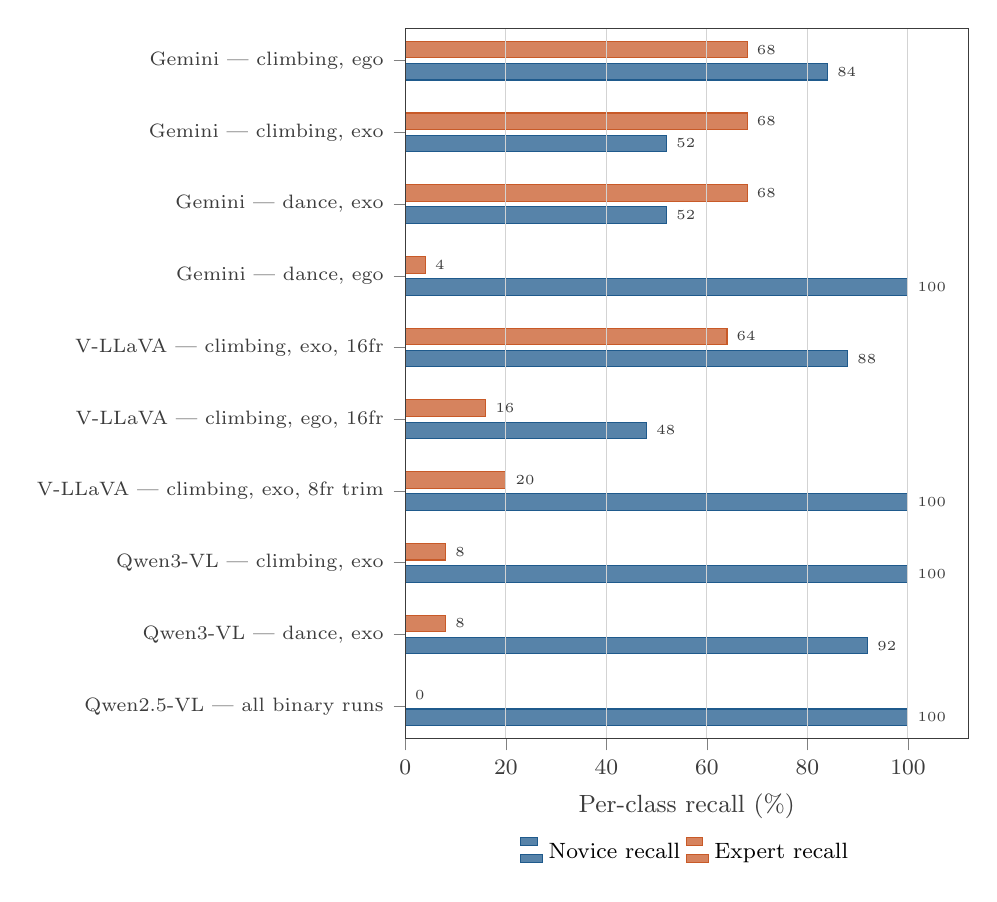
\begin{tikzpicture}
\begin{axis}[
  disshbar,
  width=0.72\textwidth, height=10.6cm,
  xmin=0, xmax=112,
  xlabel={Per-class recall (\%)},
  symbolic y coords={
    {Qwen2.5-VL --- all binary runs},
    {Qwen3-VL --- dance, exo},
    {Qwen3-VL --- climbing, exo},
    {V-LLaVA --- climbing, exo, 8fr trim},
    {V-LLaVA --- climbing, ego, 16fr},
    {V-LLaVA --- climbing, exo, 16fr},
    {Gemini --- dance, ego},
    {Gemini --- dance, exo},
    {Gemini --- climbing, exo},
    {Gemini --- climbing, ego}},
  ytick=data,
  y tick label style={font=\scriptsize},
  nodes near coords,
  every node near coord/.append style={font=\tiny},
  legend style={at={(0.5,-0.13)}, anchor=north, legend columns=2},
  bar width=6pt,
]
% --- Novice recall
\addplot[fill=cBinNovice!75, draw=cBinNovice] coordinates {
  (100,{Qwen2.5-VL --- all binary runs})
  (92,{Qwen3-VL --- dance, exo})
  (100,{Qwen3-VL --- climbing, exo})
  (100,{V-LLaVA --- climbing, exo, 8fr trim})
  (48,{V-LLaVA --- climbing, ego, 16fr})
  (88,{V-LLaVA --- climbing, exo, 16fr})
  (100,{Gemini --- dance, ego})
  (52,{Gemini --- dance, exo})
  (52,{Gemini --- climbing, exo})
  (84,{Gemini --- climbing, ego})};
% --- Expert recall
\addplot[fill=cBinExpert!75, draw=cBinExpert] coordinates {
  (0,{Qwen2.5-VL --- all binary runs})
  (8,{Qwen3-VL --- dance, exo})
  (8,{Qwen3-VL --- climbing, exo})
  (20,{V-LLaVA --- climbing, exo, 8fr trim})
  (16,{V-LLaVA --- climbing, ego, 16fr})
  (64,{V-LLaVA --- climbing, exo, 16fr})
  (4,{Gemini --- dance, ego})
  (68,{Gemini --- dance, exo})
  (68,{Gemini --- climbing, exo})
  (68,{Gemini --- climbing, ego})};
\legend{Novice recall, Expert recall}
\end{axis}
\end{tikzpicture}
\caption[Per-class recall on the binary task]{\textbf{Per-class recall on
the binary task.} Because the binary benchmark is balanced 25/25, accuracy
is the mean of the two bars; any condition whose bars sum to 100 scores
exactly 50\%, i.e.\ chance. Only Gemini on egocentric climbing (84\%
Novice, 68\% Expert) has both bars substantially above 50\%, which is what
a genuine discrimination looks like. Qwen2.5-VL sits at the degenerate
extreme, recalling every Novice and no Expert in every single binary run.}
\label{fig:binary-recall}
\end{figure}

The results highlight three key observations.

Gemini's egocentric climbing result is the only statistically significant
above-chance performance observed. Its 76\% accuracy combines 84\% Novice
recall, 68\% Expert recall and a nearly balanced prediction split of 29 to
21. This indicates that the strongest tested model can detect the simplest
proficiency distinction. Section~4.5.1 shows that this result does not
generalise across different viewpoints or activities.

Qwen2.5-VL consistently predicted ``Novice'' for every clip. This happened
in all tested conditions, including varied frame counts (8 to 64), full and
trimmed clips, egocentric and exocentric views, climbing and dance
activities, and different cameras. Its 50\% accuracy reflects the
class-balanced base rate rather than any assessment ability.

Video-LLaVA's 76\% accuracy is not comparable to Gemini's performance. For
the same clips it scored 32\% on the egocentric view, which is below
chance. Section~4.9 clarifies that the 16-frame binary prompt exceeded the
model's context window, causing silent truncation. This result therefore
cannot be considered a valid evaluation of the model's capability and is
reported only with its limitation noted.

\subsection{Four-class skill discrimination}

The four-class results are consistent across models. No model shows a
reliable above-chance result. After re-scoring, pooled accuracies are 29\%
for Gemini on climbing and 25\% on dance, while Qwen3-VL achieves 29\% and
27\% respectively. Qwen2.5-VL (24\% climbing, 28\% dance) and Video-LLaVA
(25\% on both) fall in the same band. Every model, on every activity, sits
within roughly four points of the 25\% chance baseline.

\begin{table}[H]
\centering
\caption{Climbing, representative four-class results ($n = 100$,
chance $= 25\%$).}
\label{tab:fourclass-climbing}
\footnotesize
\resizebox{\textwidth}{!}{%
\begin{tabular}{@{}l l l l r l p{3.5cm}@{}}
\toprule
\textbf{Model} & \textbf{Prompt} & \textbf{Input} & \textbf{View}
 & \textbf{Acc.} & \textbf{Recall (N/EE/IE/LE)} & \textbf{Note} \\
\midrule
Qwen3-VL & fourclass & ${\sim}1$\,fps & ego & \textbf{37\%}
  & 92 / 0 / 56 / 0 & Best four-class climbing result of any model \\
Gemini & structured & native & exo & 33\% & 40 / 0 / 92 / 0
  & Gemini's best climbing result \\
Gemini & fourclass & native & ego & 32\% & 48 / 0 / 80 / 0 & \\
Video-LLaVA & structured & 8 fr & ego, trim & 30\% & 60 / 4 / 16 / 40
  & Only run with substantial Late Expert recall \\
Qwen2.5-VL & fourclass & 16 fr & exo & 27\% & 92 / 0 / 16 / 0 & \\
Qwen3-VL & structured & ${\sim}1$\,fps & exo & 27\% & 24 / 0 / 64 / 20
  & First climbing run to predict Late Expert \\
Qwen2.5-VL & reasoning & 16 fr & exo & 18\% & 24 / 16 / 32 / 0
  & Only climbing run resolving three classes at once \\
\bottomrule
\end{tabular}}
\end{table}

\begin{table}[H]
\centering
\caption{Dance, representative four-class results ($n = 100$,
chance $= 25\%$).}
\label{tab:fourclass-dance}
\footnotesize
\resizebox{\textwidth}{!}{%
\begin{tabular}{@{}l l l l r l p{3.5cm}@{}}
\toprule
\textbf{Model} & \textbf{Prompt} & \textbf{Input} & \textbf{View}
 & \textbf{Acc.} & \textbf{Recall (N/EE/IE/LE)} & \textbf{Note} \\
\midrule
Qwen2.5-VL & structured & 16 fr & exo & \textbf{41\%} & 88 / 0 / 76 / 0
  & Best Qwen2.5-VL result of any kind \\
Qwen2.5-VL & structured & 16 fr & exo, trim & 39\% & 68 / 0 / 88 / 0
  & Close second \\
Qwen2.5-VL & fourclass & 16 fr & exo, trim & 34\% & 64 / 0 / 72 / 0 & \\
Gemini & reasoning & native & exo & 32\% & 28 / 4 / 96 / 0
  & Gemini's best dance result \\
Video-LLaVA & reasoning & 8 fr & ego, trim & 31\% & 0 / 16 / 12 / 96
  & Late-Expert-dominated, see §4.3 \\
Qwen3-VL & structured & ${\sim}1$\,fps & exo & 30\% & 12 / 4 / 80 / 24
  & Best Qwen3-VL dance result \\
\bottomrule
\end{tabular}}
\end{table}

The per-class results reveal a different pattern of model performance. The
``Early Expert'' class is almost never correctly identified by any model,
with recall of zero in nearly every run. The only exception is the
re-parsed Qwen2.5-VL reasoning run at 16\%, which remains below chance at
18\% overall accuracy. Similarly, the ``Late Expert'' class shows minimal
improvement. Gemini on climbing never predicts either Expert class in any
four-class, structured or reasoning run, instead limiting its predictions
to Novice and Intermediate Expert.

The strongest result is 41\% accuracy on dance, achieved by Qwen2.5-VL
using the structured prompt with 16 frames from an exocentric viewpoint. It
has per-class recalls of 88\% Novice, 0\% Early Expert, 76\% Intermediate
Expert and 0\% Late Expert. Similarly, Qwen3-VL achieves 37\% on climbing
with per-class recalls of 92 / 0 / 56 / 0. Both models predict only two of
the four labels, scoring zero on the others.

Figure~\ref{fig:confusion} makes the underlying independence explicit. It
shows, for each true skill level, the distribution of labels Gemini
actually predicts on climbing, pooled over all three four-way prompts. If
the model were discriminating, the four bars would differ markedly from row
to row. Instead they are close to identical.

% ------------------------------ FIGURE: confusion as stacked bars ----
\begin{figure}[H]
\centering
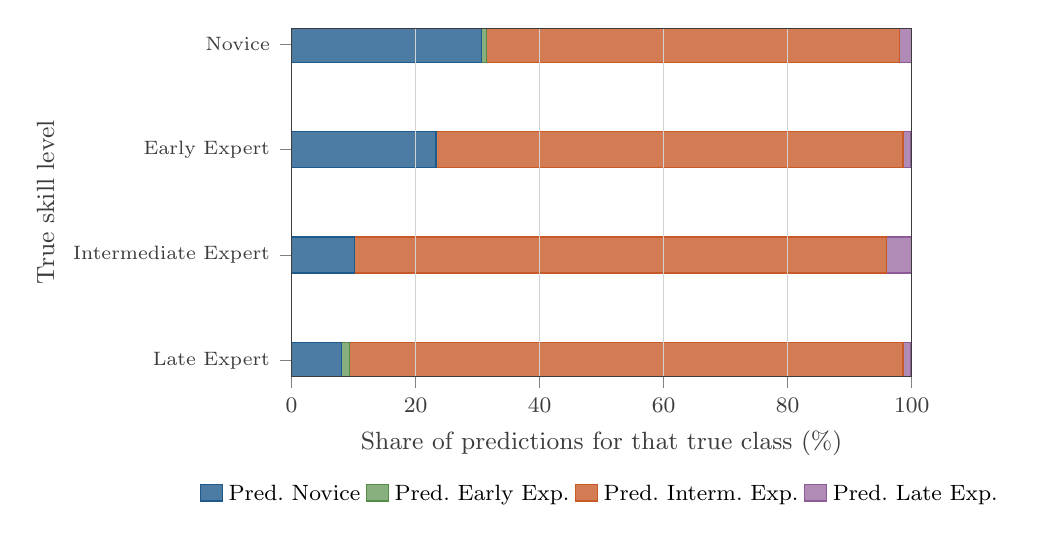
\begin{tikzpicture}
\begin{axis}[
  disshbar,
  xbar stacked,
  width=0.78\textwidth, height=6.0cm,
  xmin=0, xmax=100,
  xlabel={Share of predictions for that true class (\%)},
  symbolic y coords={{Late Expert},{Intermediate Expert},{Early Expert},{Novice}},
  ytick=data,
  y tick label style={font=\scriptsize},
  ylabel={True skill level},
  legend style={at={(0.5,-0.28)}, anchor=north, legend columns=4},
  bar width=13pt,
]
\addplot[fill=cGemini!80, draw=cGemini , bar shift=0pt] coordinates {
  (8.0,{Late Expert}) (10.1,{Intermediate Expert}) (23.3,{Early Expert}) (30.7,{Novice})};
\addplot[fill=cQwen3!70, draw=cQwen3 , bar shift=0pt] coordinates {
  (1.3,{Late Expert}) (0.0,{Intermediate Expert}) (0.0,{Early Expert}) (0.7,{Novice})};
\addplot[fill=cQwen25!80, draw=cQwen25 , bar shift=0pt] coordinates {
  (89.3,{Late Expert}) (85.9,{Intermediate Expert}) (75.3,{Early Expert}) (66.7,{Novice})};
\addplot[fill=cVLLaVA!70, draw=cVLLaVA , bar shift=0pt] coordinates {
  (1.3,{Late Expert}) (4.0,{Intermediate Expert}) (1.3,{Early Expert}) (2.0,{Novice})};
\legend{Pred.\ Novice, Pred.\ Early Exp., Pred.\ Interm.\ Exp., Pred.\ Late Exp.}
\end{axis}
\end{tikzpicture}
\caption[Predicted-label distribution by true class]{\textbf{Predicted-label
distribution by true class: Gemini, climbing, four-way prompts pooled
($n \approx 150$ valid answers per row).} Each bar is one row of a
row-normalised confusion matrix. The rows are nearly identical, which is to
say the predicted distribution barely responds to the true skill level:
Gemini labels 86--89\% of Intermediate and Late Expert climbers
``Intermediate Expert'' --- and 67\% of true novices the same way. Early
Expert is essentially never predicted at all.}
\label{fig:confusion}
\end{figure}

% ---------------------------------------------------------------------
\section{The failure is label collapse, not noise}
% ---------------------------------------------------------------------

\runin{Hypothesis (H2).} The observed failure is primarily label
collapse rather than random guessing.

\runin{Test.} Predicted-label distributions and per-class accuracies
were analysed across all experimental conditions, using the uniform
collapse criterion defined in §4.1.

\runin{Verdict.} H2 is supported. The models do not randomly guess.
Instead, they respond in the same way regardless of the input. On a
balanced benchmark, this constant answer produces chance-level accuracy.

Approximately 43\% of the tested conditions show total or near-total label
collapse, with the model assigning a single label to between 87\% and 100\%
of clips. Table~\ref{tab:collapse-prevalence} breaks this down by model.
Qwen2.5-VL predicts ``Novice'' for essentially all 50 clips in every binary
condition, consistently scoring 50.0\%. Chi-squared goodness-of-fit tests
produce $p$-values below $10^{-20}$ in the most extreme cases. Collapse is
therefore not a marginal effect but the dominant pattern in the experiment.

\begin{table}[H]
\centering
\caption{Prevalence of label collapse by model. A condition is one
model $\times$ activity $\times$ prompt $\times$ view $\times$ frame count
$\times$ trim cell. Totals are sensitive to how jointly reported ego and
exo cells are individuated and should be read as close approximations.}
\label{tab:collapse-prevalence}
\small
\begin{tabular}{@{}l r r r@{}}
\toprule
\textbf{Model} & \textbf{Conditions} & \textbf{Collapsed}
 & \textbf{\% collapsed} \\
\midrule
Video-LLaVA-7B & 49  & 28 & 57.1\% \\
Qwen2.5-VL-7B  & 89  & 42 & 47.2\% \\
Qwen3-VL-8B    & 18  &  4 & 22.2\% \\
Gemini         & 16  &  0 &  0.0\% \\
\midrule
All models     & 172 & 74 & 43.0\% \\
\bottomrule
\end{tabular}
\end{table}

Figure~\ref{fig:collapse} shows the same phenomenon on a continuous scale
rather than a binary criterion, by reporting the share of clips receiving
whichever label the model most often produced. Two observations follow.

Robustness to label collapse differs significantly by model, and does not
depend only on model size. Gemini never collapses in any of its 16
conditions, while Video-LLaVA collapses in more than half of its 49.
Video-LLaVA-7B collapses more than Qwen2.5-VL-7B despite having the same
parameter count, which is due in part to its far more limited context
capacity.

This tendency should not, however, be mistaken for capability. Although
Gemini collapses in zero conditions, it still underperforms on the
four-class task: its best climbing result is 33\%, with 0\% recall on both
Early and Late Expert.

% ------------------------------ FIGURE: collapse severity ------------
\begin{figure}[H]
\centering
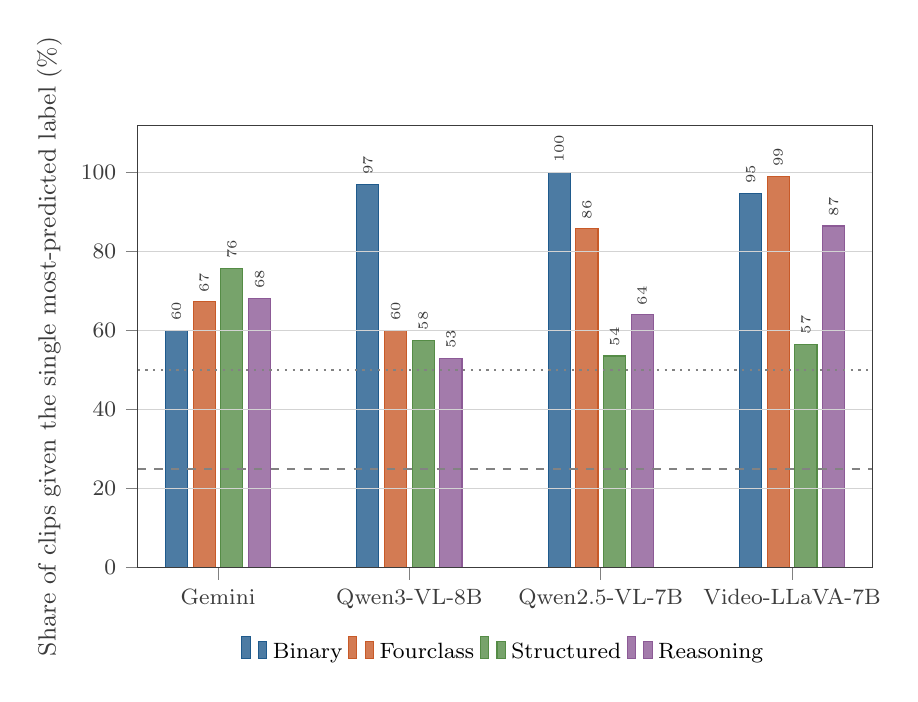
\begin{tikzpicture}
\begin{axis}[
  dissbar,
  width=0.9\textwidth, height=7.2cm,
  ymin=0, ymax=112,
  ylabel={Share of clips given the single most-predicted label (\%)},
  symbolic x coords={Gemini, {Qwen3-VL-8B}, {Qwen2.5-VL-7B}, {Video-LLaVA-7B}},
  xtick=data,
  x tick label style={font=\footnotesize},
  bar width=8pt,
  nodes near coords,
  every node near coord/.append style={font=\tiny, rotate=90, anchor=west},
  legend style={at={(0.5,-0.14)}, anchor=north, legend columns=4},
]
\addplot[fill=cGemini!80, draw=cGemini] coordinates {
  (Gemini,60.0) ({Qwen3-VL-8B},97.0) ({Qwen2.5-VL-7B},100.0) ({Video-LLaVA-7B},94.8)};
\addplot[fill=cQwen25!80, draw=cQwen25] coordinates {
  (Gemini,67.3) ({Qwen3-VL-8B},60.0) ({Qwen2.5-VL-7B},85.8) ({Video-LLaVA-7B},99.1)};
\addplot[fill=cQwen3!80, draw=cQwen3] coordinates {
  (Gemini,75.8) ({Qwen3-VL-8B},57.6) ({Qwen2.5-VL-7B},53.6) ({Video-LLaVA-7B},56.6)};
\addplot[fill=cVLLaVA!80, draw=cVLLaVA] coordinates {
  (Gemini,68.2) ({Qwen3-VL-8B},53.0) ({Qwen2.5-VL-7B},64.0) ({Video-LLaVA-7B},86.5)};
\draw[cChance, dashed, thick]
  ({rel axis cs:0,0}|-{axis cs:Gemini,25}) -- ({rel axis cs:1,0}|-{axis cs:Gemini,25});
\draw[cChance, dotted, thick]
  ({rel axis cs:0,0}|-{axis cs:Gemini,50}) -- ({rel axis cs:1,0}|-{axis cs:Gemini,50});
\legend{Binary, Fourclass, Structured, Reasoning}
\end{axis}
\end{tikzpicture}
\caption[Label-collapse severity across models and prompts]{\textbf{Label-collapse
severity across models, activities and prompt formats.} Each bar reports the
share of clips receiving the most-predicted label, averaged over climbing
and dance. A model spreading its answers evenly would sit on the dashed
line (25\%, four-label prompts) or the dotted line (50\%, binary). Bars
approaching 100\% mean one answer for nearly every clip. Binary is the most
collapse-prone format for three of the four models, and Qwen2.5-VL reaches
a full 100\% on it.}
\label{fig:collapse}
\end{figure}

% ---------------------------------------------------------------------
\section{The visual input is not the cause}
% ---------------------------------------------------------------------

Sections~4.2 and 4.3 show that the failure is consistent rather than
random. A natural explanation is that the models are not receiving enough
of the relevant visual content. Two ablations test this directly.

\subsection{Frame budget}

\runin{Hypothesis (H3).} Increasing the number of frames will improve
accuracy, because more frames provide more visual evidence.

\runin{Test.} Qwen2.5-VL was evaluated with 8 and 16 frames, with an
additional 64-frame condition. Video-LLaVA was tested at 8 and 16 frames.
This comparison is specific to Group~1, because the duration-proportional
models were never evaluated at a fixed frame count (§3.3).

\runin{Verdict.} H3 is not supported. Increasing the number of frames
does not improve performance.

For Qwen2.5-VL, increasing the frame count from 8 to 16 does not
meaningfully affect four-class accuracy, and the binary result remains a
100\% Novice collapse at both counts. The 64-frame condition, at eight
times the standard budget, does not improve binary performance either;
four-class accuracy stays between 20\% and 32\%. The one notable exception
is climbing's reasoning-exocentric condition, which improves from 18\% at
both 8 and 16 frames to 32\% at 64 frames. On dance, moving to 64 frames
produced results that were flat or worse than at 8 or 16 frames: the
highest overall accuracy of 41\%, achieved by the structured-exocentric
condition at 16 frames, drops to 27\% at 64. The frame-count effect is
therefore specific to a particular activity and prompt, rather than a
general benefit of supplying more visual information. For Video-LLaVA,
increasing the frame count failed outright for architectural reasons
detailed in §4.9.

It is also worth noting \emph{how} the one improvement happened. At 8 and
16 frames the climbing reasoning-exo run is Novice-leaning; at 64 frames
Novice is never predicted at all and the distribution becomes
Early/Intermediate-dominant. More frames changed \emph{what} the model
defaults to, not \emph{whether} it defaults.

% ------------------------------ FIGURE: frame count ------------------
\begin{figure}[H]
\centering
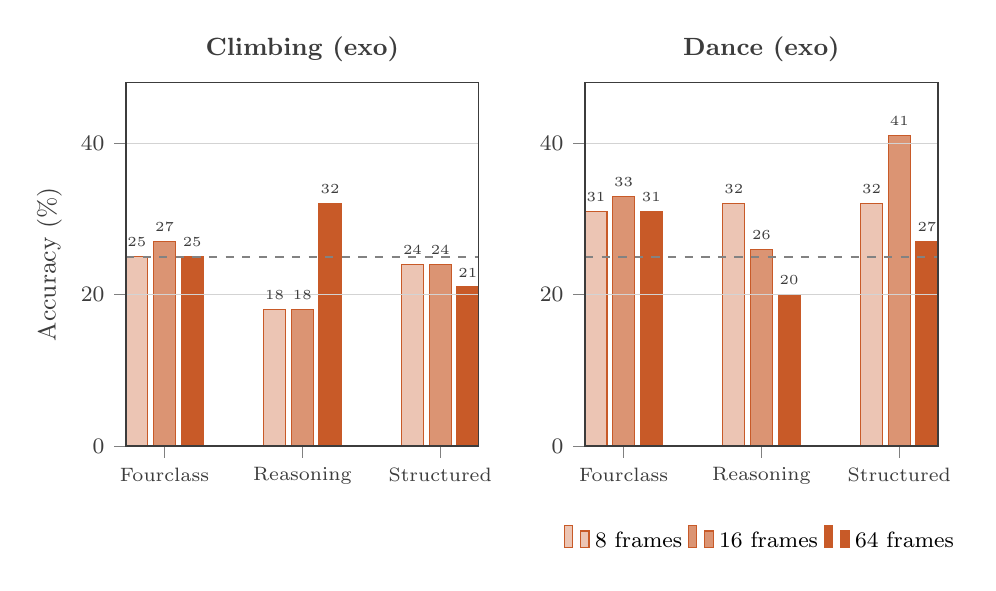
\begin{tikzpicture}
\begin{groupplot}[
  dissbar,
  group style={group size=2 by 1, horizontal sep=1.35cm},
  width=0.50\textwidth, height=6.2cm,
  ymin=0, ymax=48,
  symbolic x coords={Fourclass, Reasoning, Structured},
  xtick=data,
  x tick label style={font=\scriptsize},
  dissgroupbarwidth,
  nodes near coords,
  every node near coord/.append style={font=\tiny},
]
\nextgroupplot[title={Climbing (exo)}, ylabel={Accuracy (\%)}]
  \addplot[fill=cQwen25!35, draw=cQwen25] coordinates {
    (Fourclass,25) (Reasoning,18) (Structured,24)};
  \addplot[fill=cQwen25!65, draw=cQwen25] coordinates {
    (Fourclass,27) (Reasoning,18) (Structured,24)};
  \addplot[fill=cQwen25, draw=cQwen25] coordinates {
    (Fourclass,25) (Reasoning,32) (Structured,21)};
  \draw[cChance, dashed, thick]
    ({rel axis cs:0,0}|-{axis cs:Fourclass,25}) --
    ({rel axis cs:1,0}|-{axis cs:Fourclass,25});
\nextgroupplot[title={Dance (exo)}, legend style={at={(0.5,-0.20)},
               anchor=north, legend columns=3}]
  \addplot[fill=cQwen25!35, draw=cQwen25] coordinates {
    (Fourclass,31) (Reasoning,32) (Structured,32)};
  \addplot[fill=cQwen25!65, draw=cQwen25] coordinates {
    (Fourclass,33) (Reasoning,26) (Structured,41)};
  \addplot[fill=cQwen25, draw=cQwen25] coordinates {
    (Fourclass,31) (Reasoning,20) (Structured,27)};
  \draw[cChance, dashed, thick]
    ({rel axis cs:0,0}|-{axis cs:Fourclass,25}) --
    ({rel axis cs:1,0}|-{axis cs:Fourclass,25});
  \legend{8 frames, 16 frames, 64 frames}
\end{groupplot}
\end{tikzpicture}
\caption[Effect of sampled frame count]{\textbf{Effect of sampled frame
count (Qwen2.5-VL-7B, entire clip, exocentric view).} The dashed line is
the 25\% four-class chance baseline. Eight-fold more frames produces no
systematic gain: on climbing only the reasoning prompt moves
(18\%\,$\rightarrow$\,32\%), and on dance every prompt is flat or worse at
64 frames, including the project's best Qwen2.5-VL result
(41\%\,$\rightarrow$\,27\%). The one improvement does not replicate across
activities, so it is not evidence that more visual evidence helps.}
\label{fig:frames}
\end{figure}

\subsection{Temporal trimming}

\runin{Hypothesis (H4).} Removing idle or off-activity footage by
trimming to the annotated task window will improve accuracy.

\runin{Test.} Every Group~1 condition was run twice, once on the entire
clip and once on the clip trimmed to the annotated
\texttt{task\_start\_sec}--\texttt{task\_end\_sec} window.

\runin{Verdict.} H4 is not supported. Trimming improves accuracy about
as often as it reduces it.

When the model is provided with individual frames from a known Late Expert
clip, it answers ``Novice'' for a person who is standing or looking at a
route, but scores higher for frames of active climbing. Uniform sampling
across a full clip includes mostly frames other than peak execution, which
motivated the trimming experiment.

Qwen2.5-VL and Video-LLaVA binary runs remain almost 100\% Novice-collapsed
after trimming in every condition. Figure~\ref{fig:trim} shows that the
difference varies by up to 13 points between paired ego and exo views
of the \emph{same} clips. The Video-LLaVA climbing structured condition
drops from 28.6\% to 15.3\% on the exo view, while the Qwen2.5-VL
dance structured result shows the same pattern at a smaller scale, dropping
from 41\% to 39\% at 16 frames. These findings indicate that the Novice
bias persists despite the removal of the idle frames assumed to cause it.

The effect of trimming is unpredictable, because it also produced notable
single-view improvements. Video-LLaVA's climbing structured result
increased by 5.3 points in the egocentric view, and its dance structured
result by 7.0 points in the exocentric view. However, these do not
represent a consistent overall effect: the climbing egocentric improvement
was not matched in the exocentric view of the same clips, which instead
decreased by 13.3 points. A genuine reduction in input noise should not
help one camera and hurt another on identical footage.

% ------------------------------ FIGURE: trimming deltas --------------
\begin{figure}[H]
\centering
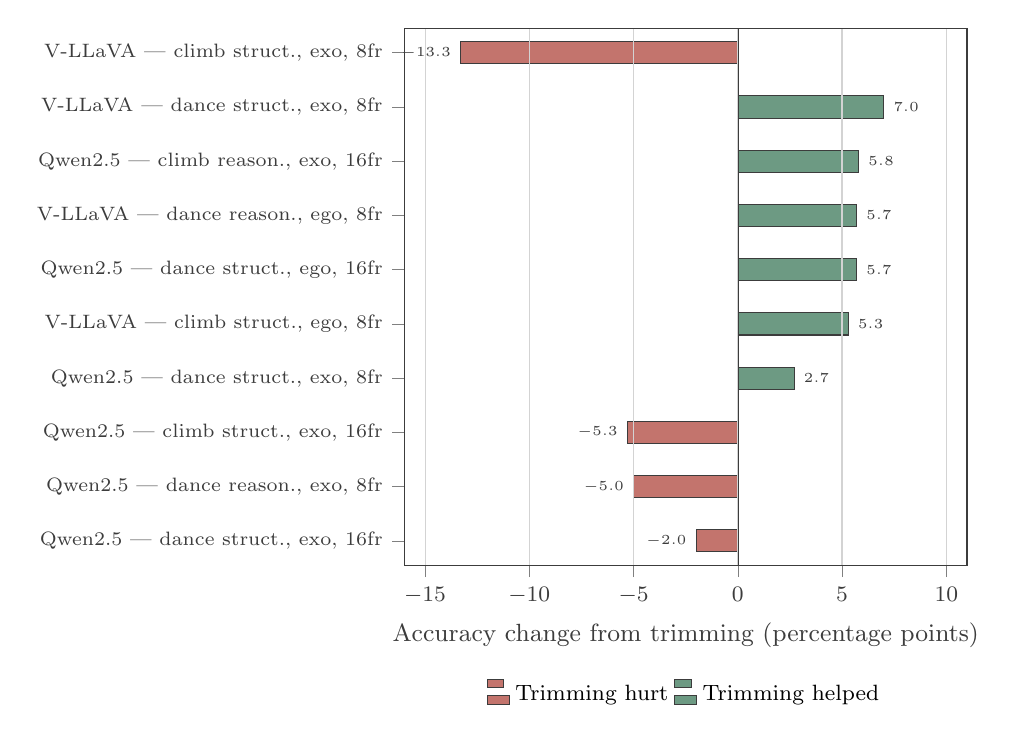
\begin{tikzpicture}
\begin{axis}[
  disshbar,
  width=0.72\textwidth, height=8.4cm,
  xmin=-16, xmax=11,
  xlabel={Accuracy change from trimming (percentage points)},
  symbolic y coords={
    {Qwen2.5 --- dance struct., exo, 16fr},
    {Qwen2.5 --- dance reason., exo, 8fr},
    {Qwen2.5 --- climb struct., exo, 16fr},
    {Qwen2.5 --- dance struct., exo, 8fr},
    {V-LLaVA --- climb struct., ego, 8fr},
    {Qwen2.5 --- dance struct., ego, 16fr},
    {V-LLaVA --- dance reason., ego, 8fr},
    {Qwen2.5 --- climb reason., exo, 16fr},
    {V-LLaVA --- dance struct., exo, 8fr},
    {V-LLaVA --- climb struct., exo, 8fr}},
  ytick={
    {Qwen2.5 --- dance struct., exo, 16fr},
    {Qwen2.5 --- dance reason., exo, 8fr},
    {Qwen2.5 --- climb struct., exo, 16fr},
    {Qwen2.5 --- dance struct., exo, 8fr},
    {V-LLaVA --- climb struct., ego, 8fr},
    {Qwen2.5 --- dance struct., ego, 16fr},
    {V-LLaVA --- dance reason., ego, 8fr},
    {Qwen2.5 --- climb reason., exo, 16fr},
    {V-LLaVA --- dance struct., exo, 8fr},
    {V-LLaVA --- climb struct., exo, 8fr}},
  y tick label style={font=\scriptsize},
  bar width=8pt,
  nodes near coords,
  nodes near coords style={/pgf/number format/precision=1,
                           /pgf/number format/fixed,
                           /pgf/number format/fixed zerofill},
  every node near coord/.append style={font=\tiny},
  legend style={at={(0.5,-0.20)}, anchor=north, legend columns=2},
]
\addplot[draw=cInk, fill=cNeg!75, bar shift=0pt] coordinates {
  (-2.0,{Qwen2.5 --- dance struct., exo, 16fr})
  (-5.0,{Qwen2.5 --- dance reason., exo, 8fr})
  (-5.3,{Qwen2.5 --- climb struct., exo, 16fr})
  (-13.3,{V-LLaVA --- climb struct., exo, 8fr})};
\addplot[draw=cInk, fill=cPos!75, bar shift=0pt] coordinates {
  (2.7,{Qwen2.5 --- dance struct., exo, 8fr})
  (5.3,{V-LLaVA --- climb struct., ego, 8fr})
  (5.7,{Qwen2.5 --- dance struct., ego, 16fr})
  (5.7,{V-LLaVA --- dance reason., ego, 8fr})
  (5.8,{Qwen2.5 --- climb reason., exo, 16fr})
  (7.0,{V-LLaVA --- dance struct., exo, 8fr})};
\draw[cInk, thick]
  ({axis cs:0,{Qwen2.5 --- dance struct., exo, 16fr}}|-{rel axis cs:0,0})
  -- ({axis cs:0,{Qwen2.5 --- dance struct., exo, 16fr}}|-{rel axis cs:0,1});
\legend{Trimming hurt, Trimming helped}
\end{axis}
\end{tikzpicture}
\caption[Effect of trimming to the annotated task window]{\textbf{Effect of
trimming to the annotated task window: the ten largest changes.} Bars to the
right of zero are conditions where trimming helped, bars to the left where
it hurt. The distribution is close to symmetric, which is what ``no
effect'' looks like on a noisy measurement. The decisive pair is
Video-LLaVA climbing structured: the \emph{same} clips trimmed the
\emph{same} way gain 5.3 points on the egocentric camera and lose 13.3 on
the exocentric one. Removing genuinely irrelevant footage should not do
that.}
\label{fig:trim}
\end{figure}

% ---------------------------------------------------------------------
\section{Viewpoint and benchmark scale}
% ---------------------------------------------------------------------

\subsection{Viewpoint}

\runin{Hypothesis (H5).} Exocentric viewpoint will outperform
egocentric viewpoint, because it shows whole-body posture directly relevant
to skill assessment, whereas egocentric shows mainly hands and the
immediate surroundings.

\runin{Test.} Both viewpoint runs were paired on identical clips,
prompts and frame budgets.

\runin{Verdict.} H5 is not supported. Exocentric viewpoint does not
consistently outperform egocentric viewpoint; the direction depends on both
the model and the activity.

Gemini's results contradict the hypothesis outright. It achieved 76\%
binary accuracy on egocentric climbing clips compared with 60\% on
exocentric. The same model on dance shows the opposite pattern, with
exocentric outperforming egocentric (60\% versus 52\%). A fixed mechanism
of the kind the hypothesis proposes cannot explain an activity-dependent
reversal.

Qwen2.5-VL shows a different pattern. Egocentric input strengthens the
model's Novice default rather than reducing accuracy through lost detail.
Novice predictions increase from 75\% to 85\% on climbing and from 36\% to
90\% on dance under egocentric framing. Every reliable Qwen2.5-VL result in
this chapter comes from an exocentric view. This does not indicate that
exocentric input is inherently more informative; rather, it appears to be
less prone to collapse. For instance, exocentric accuracy on the dance
structured task is 41\%, but the corresponding egocentric result collapses
to exactly 25\%. The finding matches the direction predicted by the
hypothesis but not the mechanism behind it: the exocentric advantage is not
that it shows more of the body, but that the egocentric view is more likely
to trigger collapse.

% ------------------------------ FIGURE: viewpoint --------------------
\begin{figure}[H]
\centering
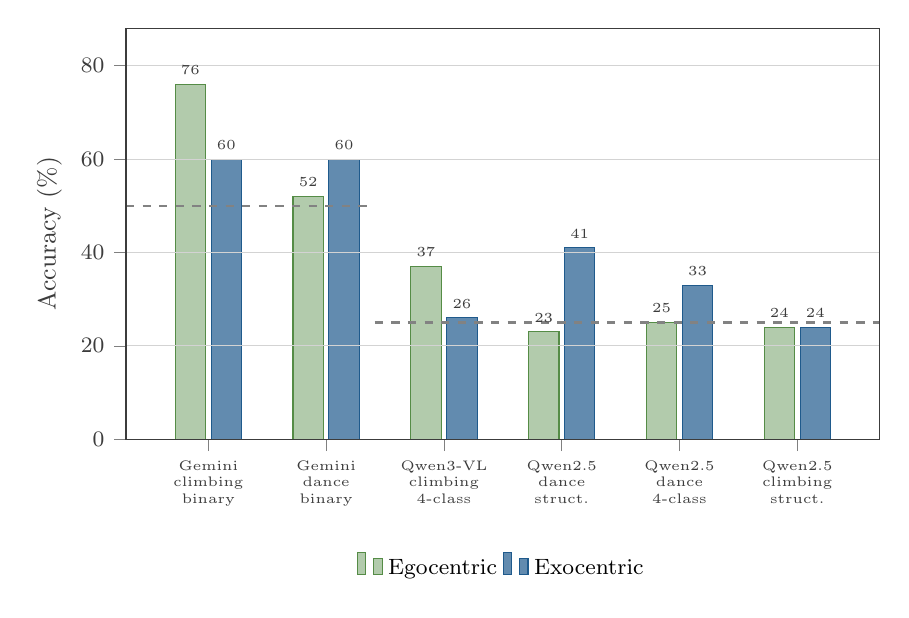
\begin{tikzpicture}
\begin{axis}[
  dissbar,
  width=0.92\textwidth, height=6.8cm,
  ymin=0, ymax=88,
  ylabel={Accuracy (\%)},
  symbolic x coords={GemClimbB, GemDanceB, Q3ClimbF, Q25DanceS,
                     Q25DanceF, Q25ClimbS},
  xtick=data,
  xticklabels={
    {Gemini\\climbing\\binary},
    {Gemini\\dance\\binary},
    {Qwen3-VL\\climbing\\4-class},
    {Qwen2.5\\dance\\struct.},
    {Qwen2.5\\dance\\4-class},
    {Qwen2.5\\climbing\\struct.}},
  x tick label style={font=\tiny, align=center},
  bar width=11pt,
  nodes near coords,
  every node near coord/.append style={font=\tiny},
  legend style={at={(0.5,-0.26)}, anchor=north, legend columns=2},
]
\addplot[fill=cQwen3!45, draw=cQwen3] coordinates {
  (GemClimbB,76) (GemDanceB,52) (Q3ClimbF,37)
  (Q25DanceS,23) (Q25DanceF,25) (Q25ClimbS,24)};
\addplot[fill=cGemini!70, draw=cGemini] coordinates {
  (GemClimbB,60) (GemDanceB,60) (Q3ClimbF,26)
  (Q25DanceS,41) (Q25DanceF,33) (Q25ClimbS,24)};
\draw[cChance, dashed, thick]
  ({rel axis cs:0,0}|-{axis cs:GemClimbB,50}) --
  ({rel axis cs:0.33,0}|-{axis cs:GemClimbB,50});
\draw[cChance, dashed, thick]
  ({rel axis cs:0.33,0}|-{axis cs:GemClimbB,25}) --
  ({rel axis cs:1,0}|-{axis cs:GemClimbB,25});
\legend{Egocentric, Exocentric}
\end{axis}
\end{tikzpicture}
\caption[Effect of camera viewpoint]{\textbf{Effect of camera viewpoint on
paired runs (identical clips, prompts and frame budgets).} The dashed lines
mark the relevant chance baseline --- 50\% for the two binary conditions on
the left, 25\% for the four-class conditions on the right. The direction of
the viewpoint effect reverses between models and between activities:
Gemini prefers ego on climbing and exo on dance, while Qwen2.5-VL's
exocentric advantage on dance is an escape from collapse rather than a gain
from better body visibility. No single viewpoint is reliably better.}
\label{fig:viewpoint}
\end{figure}

\subsection{Benchmark scale}

A final check excludes a small-sample artefact. The benchmark was rebuilt
at approximately 100 clips per class ($n = 389$, with Late Expert capped at
89 by data availability) and re-run at 8 frames.

\begin{table}[H]
\centering
\caption{Small-sample against large-sample comparison, Qwen2.5-VL-7B,
climbing, 8 frames, entire clip.}
\label{tab:scale}
\small
\begin{tabular}{@{}l l r r r@{}}
\toprule
\textbf{Prompt} & \textbf{View} & \textbf{$n = 100$} & \textbf{$n = 389$}
 & \textbf{Delta} \\
\midrule
Reasoning  & exo & 18.0\%             & 16.7\%             & $-1.3$ \\
Structured & exo & 24.0\%             & 23.4\%             & $-0.6$ \\
Reasoning  & ego & 24.0\% (collapsed) & 25.4\% (collapsed) & $+1.4$ \\
Structured & ego & 19.0\%             & 25.4\%             & $+6.4$ \\
\bottomrule
\end{tabular}
\end{table}

The same pattern holds at roughly four times the sample size. Egocentric
views still collapse and exocentric views partially resolve. Three of the
four conditions fall within 1.4 points of the original figures. The
reasoning-egocentric condition remains collapsed, predicting Novice for 382
of 389 clips. These findings are not a sampling artefact.

% ---------------------------------------------------------------------
\section{Generalisation across activity domains}
% ---------------------------------------------------------------------

The remaining plausible explanation is that bouldering is especially hard
to judge, or that its annotations are unusually noisy.

\runin{Hypothesis (H6).} Performance will differ meaningfully across
activities (climbing, dance, basketball, JIGSAWS, mixed-activity).

\runin{Test.} The evaluation was extended to basketball from EgoExo4D,
to a mixed benchmark pooling basketball, music, cooking and soccer with
climbing and dance excluded by design, and to JIGSAWS robotic suturing as
an out-of-distribution dataset recorded with a single close-range camera
and requiring a domain-specific rephrased prompt.

\runin{Verdict.} H6 is not supported. Every domain tested showed the
collapse.

\begin{table}[H]
\centering
\caption{Cross-domain and cross-dataset results, Qwen2.5-VL-7B, 8 frames.}
\label{tab:crossdomain}
\footnotesize
\resizebox{\textwidth}{!}{%
\begin{tabular}{@{}l l l r r l p{3.4cm}@{}}
\toprule
\textbf{Test} & \textbf{Format} & \textbf{View} & \textbf{Acc.}
 & \textbf{Chance} & \textbf{Distribution} & \textbf{Reading} \\
\midrule
Basketball (EgoExo4D) & binary & ego+exo & 24.0\% & 50\%
  & Novice 34, Unknown 16
  & Below chance ($p = 0.0003$); 16/50 rows unparseable from missing video,
    15 on Expert-labelled clips \\
\addlinespace
JIGSAWS suturing & binary & exo & 65.5\% & 50\% & Novice 29/29
  & Not signal; majority-class artefact of a 19\,N / 10\,E imbalance;
    $p = 0.136$ \\
\addlinespace
Mixed activity & binary & ego+exo & 25.0\% & 50\% & Novice 100/100
  & Collapsed; far below chance \\
\addlinespace
Mixed activity & structured & exo & 19.0\% & 25\%
  & IE 51, N 44, Unk 5 & Kept; below chance \\
\addlinespace
Mixed activity & structured & ego & 23.0\% & 25\%
  & IE 48, Unk 27, N 25 & Kept; at chance \\
\bottomrule
\end{tabular}}
\end{table}

The failure holds across seven distinct activity types --- bouldering,
dance, basketball, surgical suturing, music, cooking and soccer --- spanning
two datasets.

\subsection{JIGSAWS}

At 65.5\%, JIGSAWS is the highest cross-domain score in the study, and the
only one above chance. But it was produced by a model that answered
``Novice'' 29 times out of 29. Per-class accuracy is 100\% on Novice and
0\% on Expert. The result is not statistically significant: a binomial test
gives $p = 0.136$. If the benchmark had contained an equal mix of classes,
this same behaviour would have scored 50\%; had it been mostly Expert
clips, it would have scored 34.5\%. The accuracy score reflects how the
benchmark is balanced, not how well the model is performing. This is the
single clearest justification for the reporting convention of §4.1.

\subsection{A mixed-activity benchmark}

The mixed-activity structured runs show uneven results across activities:
basketball and cooking retain more signal than music and soccer.

\begin{table}[H]
\centering
\caption{Per-activity accuracy within the mixed benchmark, structured
prompt, 8 frames, trimmed.}
\label{tab:mixed-activity}
\small
\begin{tabular}{@{}l r r r r@{}}
\toprule
\textbf{Activity} & \textbf{$n$} & \textbf{Correct (exo)}
 & \textbf{Correct (ego)} & \textbf{Combined rate} \\
\midrule
Basketball    & 48 & 12 & 9 & 21.9\% \\
Cooking       & 21 &  5 & 8 & 31.0\% \\
Music (piano) & 20 &  2 & 5 & 17.5\% \\
Soccer        & 11 &  0 & 1 &  4.5\% \\
\bottomrule
\end{tabular}
\end{table}

One possible explanation is that whatever weak signal remains tends to
align with activities involving clear, visible interactions with objects
--- a ball being handled, a knife being used --- where success or failure
can be inferred from a single frame. This contrasts with activities relying
on whole-body motion or precise motor timing. The idea is consistent with
the diagnosis in §4.7. It must, however, be treated as speculative: sample
sizes range from 11 to 48, the differences are untested for significance,
and all accuracies are at or below chance, so the comparison is between two
kinds of failure rather than between success and failure. It is offered as
a hypothesis for future work, not as a finding.

% ------------------------------ FIGURE: cross-domain -----------------
\begin{figure}[H]
\centering
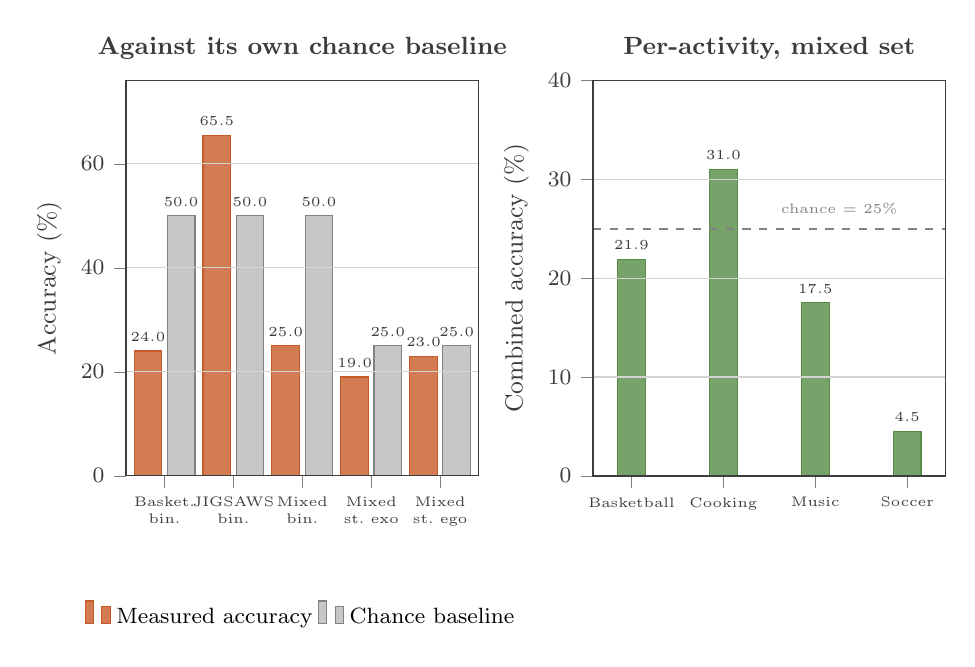
\begin{tikzpicture}
\begin{groupplot}[
  dissbar,
  group style={group size=2 by 1, horizontal sep=1.45cm},
  width=0.50\textwidth, height=6.6cm,
  ymin=0, ymax=76,
  dissgroupbarwide,
  nodes near coords,
  nodes near coords style={/pgf/number format/precision=1,
                           /pgf/number format/fixed,
                           /pgf/number format/fixed zerofill},
  every node near coord/.append style={font=\tiny},
]
\nextgroupplot[
  title={Against its own chance baseline},
  ylabel={Accuracy (\%)},
  symbolic x coords={BasketB, JigsawsB, MixedB, MixedSX, MixedSE},
  xtick=data,
  xticklabels={
    {Basket.\\bin.},
    {JIGSAWS\\bin.},
    {Mixed\\bin.},
    {Mixed\\st.\ exo},
    {Mixed\\st.\ ego}},
  x tick label style={font=\tiny, align=center},
  legend style={at={(0.5,-0.30)}, anchor=north, legend columns=2},
]
  \addplot[fill=cQwen25!80, draw=cQwen25] coordinates {
    (BasketB,24.0) (JigsawsB,65.5) (MixedB,25.0)
    (MixedSX,19.0) (MixedSE,23.0)};
  \addplot[fill=cChance!45, draw=cChance] coordinates {
    (BasketB,50) (JigsawsB,50) (MixedB,50)
    (MixedSX,25) (MixedSE,25)};
  \legend{Measured accuracy, Chance baseline}
\nextgroupplot[
  title={Per-activity, mixed set},
  ylabel={Combined accuracy (\%)},
  symbolic x coords={Basketball, Cooking, Music, Soccer},
  xtick=data,
  x tick label style={font=\tiny},
  ymax=40,
]
  \addplot[fill=cQwen3!80, draw=cQwen3] coordinates {
    (Basketball,21.9) (Cooking,31.0) (Music,17.5) (Soccer,4.5)};
  \draw[cChance, dashed, thick]
    ({rel axis cs:0,0}|-{axis cs:Basketball,25}) --
    ({rel axis cs:1,0}|-{axis cs:Basketball,25});
  \node[font=\tiny, color=cChance, anchor=south east]
    at (axis cs:Soccer,25.5) {chance = 25\%};
\end{groupplot}
\end{tikzpicture}
\caption[Cross-domain generalisation]{\textbf{Cross-domain generalisation
(Qwen2.5-VL-7B, 8 frames).} \emph{Left:} every cross-domain test plotted
against its own chance baseline. The only bar clearing its baseline is
JIGSAWS, and that is the majority-class artefact of §4.6.1 --- a model that
answered ``Novice'' 29 times out of 29 on a 19/10 imbalanced set.
\emph{Right:} the per-activity breakdown inside the mixed benchmark. Only
cooking exceeds chance, on 21 clips; soccer collapses almost completely.
The comparison is between two kinds of failure, not between success and
failure.}
\label{fig:crossdomain}
\end{figure}

% ---------------------------------------------------------------------
\section{Locating the failure: perception or language?}
% ---------------------------------------------------------------------

Sections 4.4 to 4.6 exclude the input-side explanations one by one: it is
not the frame budget, not idle footage, not the camera, not the sample
size, and not the activity. What remains is to ask where inside the model
the failure occurs. Two controls answer this, and they are the most
informative experiments in the project because neither of them requires the
model to succeed at the task at all.

\subsection{Perception is intact}

A scene-content diagnostic first confirms that the models see the video.
Asked to describe what is present rather than to judge it, all four models
correctly identify the activity, the number of people, the equipment and
the dominant colours, on clips whose skill judgement they then get wrong.
Whatever is failing, it is not video decoding and it is not gross
perception.

\subsection{Vision alone succeeds (H7)}

\runin{Hypothesis (H7).} Skill-discriminative signal is present in
visual features even where language output fails.

\runin{Test.} A linear classifier was trained on frozen CLIP features
extracted from the same exocentric climbing clips, with no language
generation anywhere in the pipeline, and evaluated by 5-fold
cross-validation.

\runin{Verdict.} H7 is supported, decisively.

The linear probe reaches \textbf{67.0\%} four-class accuracy (5-fold
cross-validation; 95\% CI 62.5--71.5\%) on clips where the VLMs score
24--25\%. The
features are frozen: nothing was learned about vision, only a linear
partition of a representation the encoder already produced. The
discriminative signal for proficiency is therefore present, and linearly
accessible, in the visual representation \emph{before} it reaches any
language model. It is also worth noting that this exceeds the 47--53\%
reported by trained, task-specific supervised methods on the same
four-class benchmark, which places the result well outside the range that
could be attributed to noise.

\subsection{Language alone also fails (H8)}

\runin{Hypothesis (H8).} Skill level is recoverable from expert
language alone.

\runin{Test.} The models were given an expert's written coaching
commentary describing a climbing attempt --- no video, no frames, nothing
visual --- and asked for the same four-class judgement.

\runin{Verdict.} H8 is not supported. Text-only performance lands in
the same band as video.

Qwen2.5-VL scores 26.0\% and Video-LLaVA 33.0\% on the text-only
four-class task, against video-based bests of roughly 27\% and 30\%
respectively for the same models on climbing. Text does not fail where
video succeeds, nor does it clearly outperform video. Both text-only runs
also reproduce the same collapse asymmetry seen throughout: Qwen2.5-VL
virtually never predicts Novice from text (3 of 100), exactly as it never
does from egocentric video, while Video-LLaVA over-predicts it (35 of 100),
mirroring its video-side bias.

\subsection{What the two controls jointly establish}

Taken together the three results localise the failure precisely. Perception
is intact. A linear read-out of the visual representation classifies skill
at 67\%. Supplying the evidence in explicit expert language instead of
pixels does not help either. The bottleneck is therefore neither the
visual encoder nor the availability of the evidence: it is the step at
which either modality must be converted into the correct categorical label.
This is a within-task instance of the argument made by \citet{tong2024},
and it is the central claim of this dissertation.

% ---------------------------------------------------------------------
\section{Qualitative analysis: what the models actually say}
% ---------------------------------------------------------------------

Accuracy tables record what the models answered; this section analyses how
they answered, and identifies a distinct failure signature for each model
family.

Qwen2.5-VL under a free-text prompt frequently hedges rather than
committing to a single class, writing the literal disjunction ``novice or
early expert''. This occurred 24 times in a 16-frame trimmed climbing run,
12 times in the corresponding entire-clip run, and 11 and 7 times in the
8-frame versions, against effectively zero instances under four-class or
structured prompts. The behaviour suggests a failure to make a confident
distinction rather than calibrated uncertainty, since it concentrates on
one specific class pair and disappears entirely when the output format
forces a commitment. A representative answer, on a clip whose ground truth
is Novice, reads: \emph{the climber appears to be a novice or early expert
based on the following observations \ldots{} the climber's technique and
body alignment suggest that they are at a novice or early expert level.}
The re-parser scores such answers as \texttt{Unknown} rather than resolving
the disjunction arbitrarily, since any Early Expert credit awarded from one
would be a coin flip.

Fixed-frame models also respond stereotypically. Qwen2.5-VL opens 99.8\% of
its egocentric dance reasoning answers with the same sentence, and 86.6\%
of its egocentric climbing answers, while Video-LLaVA reuses identical
phrasing across unrelated clips. Such repetition indicates that the
response is being generated from a prior rather than from the video
content, which weakens the evidential value of the text considerably.

% ------------------------------ FIGURE: stereotypy -------------------
\begin{figure}[H]
\centering
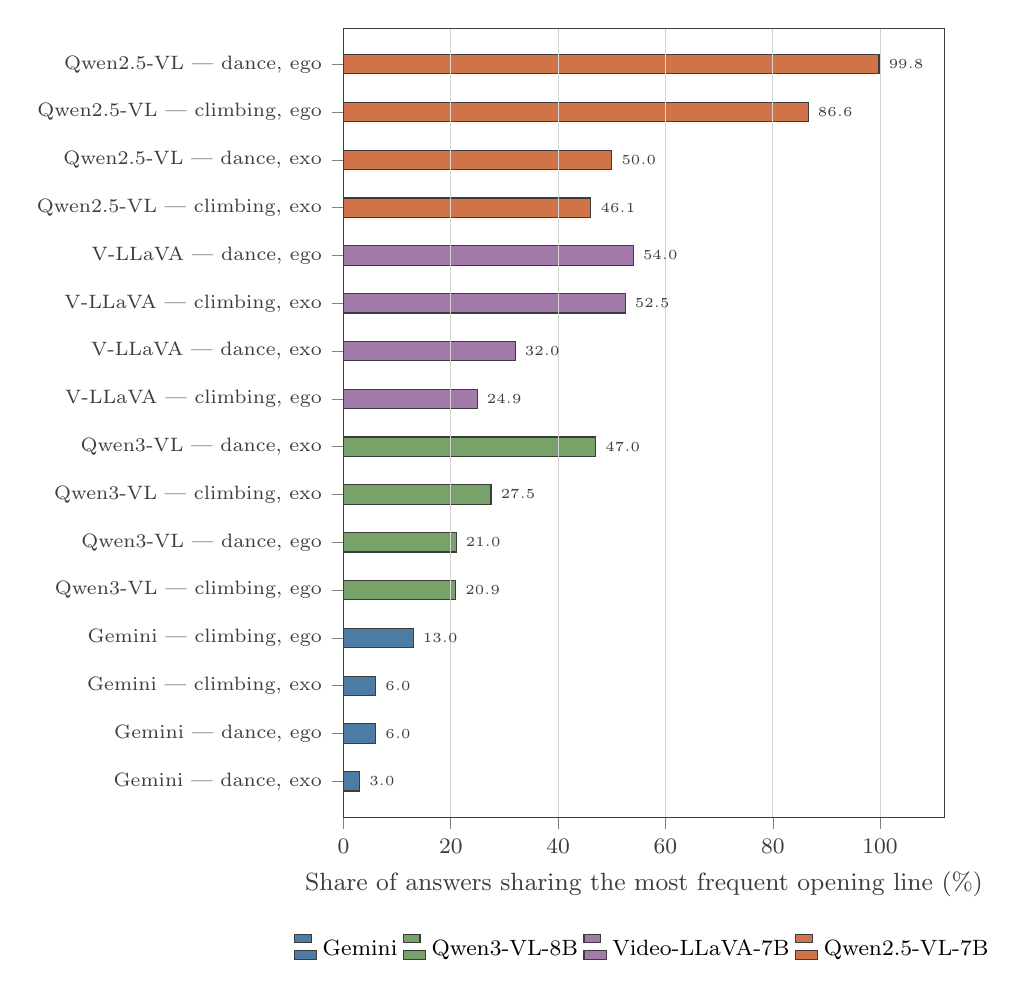
\begin{tikzpicture}
\begin{axis}[
  disshbar,
  width=0.76\textwidth, height=11.6cm,
  xmin=0, xmax=112,
  xlabel={Share of answers sharing the most frequent opening line (\%)},
  symbolic y coords={
    {Gemini --- dance, exo},
    {Gemini --- dance, ego},
    {Gemini --- climbing, exo},
    {Gemini --- climbing, ego},
    {Qwen3-VL --- climbing, ego},
    {Qwen3-VL --- dance, ego},
    {Qwen3-VL --- climbing, exo},
    {Qwen3-VL --- dance, exo},
    {V-LLaVA --- climbing, ego},
    {V-LLaVA --- dance, exo},
    {V-LLaVA --- climbing, exo},
    {V-LLaVA --- dance, ego},
    {Qwen2.5-VL --- climbing, exo},
    {Qwen2.5-VL --- dance, exo},
    {Qwen2.5-VL --- climbing, ego},
    {Qwen2.5-VL --- dance, ego}},
  ytick={
    {Gemini --- dance, exo},{Gemini --- dance, ego},
    {Gemini --- climbing, exo},{Gemini --- climbing, ego},
    {Qwen3-VL --- climbing, ego},{Qwen3-VL --- dance, ego},
    {Qwen3-VL --- climbing, exo},{Qwen3-VL --- dance, exo},
    {V-LLaVA --- climbing, ego},{V-LLaVA --- dance, exo},
    {V-LLaVA --- climbing, exo},{V-LLaVA --- dance, ego},
    {Qwen2.5-VL --- climbing, exo},{Qwen2.5-VL --- dance, exo},
    {Qwen2.5-VL --- climbing, ego},{Qwen2.5-VL --- dance, ego}},
  y tick label style={font=\scriptsize},
  bar width=7pt,
  nodes near coords,
  nodes near coords style={/pgf/number format/precision=1,
                           /pgf/number format/fixed,
                           /pgf/number format/fixed zerofill},
  every node near coord/.append style={font=\tiny},
  legend style={at={(0.5,-0.14)}, anchor=north, legend columns=4},
]
\addplot[draw=cInk, fill=cGemini!80, bar shift=0pt] coordinates {
  (3.0,{Gemini --- dance, exo}) (6.0,{Gemini --- dance, ego})
  (6.0,{Gemini --- climbing, exo}) (13.0,{Gemini --- climbing, ego})};
\addplot[draw=cInk, fill=cQwen3!80, bar shift=0pt] coordinates {
  (20.9,{Qwen3-VL --- climbing, ego}) (21.0,{Qwen3-VL --- dance, ego})
  (27.5,{Qwen3-VL --- climbing, exo}) (47.0,{Qwen3-VL --- dance, exo})};
\addplot[draw=cInk, fill=cVLLaVA!80, bar shift=0pt] coordinates {
  (24.9,{V-LLaVA --- climbing, ego}) (32.0,{V-LLaVA --- dance, exo})
  (52.5,{V-LLaVA --- climbing, exo}) (54.0,{V-LLaVA --- dance, ego})};
\addplot[draw=cInk, fill=cQwen25!85, bar shift=0pt] coordinates {
  (46.1,{Qwen2.5-VL --- climbing, exo}) (50.0,{Qwen2.5-VL --- dance, exo})
  (86.6,{Qwen2.5-VL --- climbing, ego}) (99.8,{Qwen2.5-VL --- dance, ego})};
\legend{Gemini, Qwen3-VL-8B, Video-LLaVA-7B, Qwen2.5-VL-7B}
\end{axis}
\end{tikzpicture}
\caption[Stereotypy of reasoning responses]{\textbf{Stereotypy of reasoning
responses: the share of answers in each condition beginning with the single
most frequent opening line.} A model writing genuinely per-clip text would
sit near the left edge. The fixed-frame models do not: Qwen2.5-VL opens
99.8\% of its egocentric dance answers identically, and 86.6\% of its
egocentric climbing answers. Gemini sits at 3--13\% throughout, writing
distinct prose for almost every clip --- and still, per
Figure~\ref{fig:confusion}, produces judgements nearly independent of the
ground truth. Specificity of language is not evidence of grounding.}
\label{fig:stereotypy}
\end{figure}

By contrast, the duration-proportional models produce descriptive,
clip-specific analyses running to 1{,}000--2{,}500 characters, naming
particular holds, movements and errors; at most 3--13\% of Gemini's answers
share an opening line. Despite this verbosity, the final judgement remains
poorly correlated with the ground truth, as
Figure~\ref{fig:confusion} showed. This is arguably the more dangerous of
the two failure modes, because fluent, specific, plausible prose is exactly
what a human reader uses as evidence that a model understood the video.

Occasionally Gemini refuses to answer when the video does not contain the
requested content --- for example when the camera wearer is filming other
dancers rather than dancing, or when a team is talking in a briefing rather
than climbing. Although these refusals are scored as incorrect, they are
arguably the most genuinely grounded visual behaviour observed anywhere in
the project, and they expose real noise in the egocentric ground truth,
which is systematically less reliable than the exocentric annotations.

A consistent pattern holds across models: the extreme classes are not
recognised. Recall for Early Expert is zero in most four-class conditions,
and Late Expert recall is very low except for Qwen3-VL, which shows modest
improvement. The four-level ordinal scale is effectively answered as a
two-level one, corroborating the collapse analysis of §4.3.

% ---------------------------------------------------------------------
\section{Reliability and limitations}
% ---------------------------------------------------------------------

Several constraints bound the results above and are reported here rather
than distributed through the chapter.

\runin{Video-LLaVA's context ceiling.} The 16-frame runs are not valid
evaluations of the model. At 256 visual tokens per frame,
$16 \times 256 = 4{,}096$ tokens fill the entire Vicuna-7B context window
before any prompt text is added. The structured and reasoning scripts abort
generation on an explicit guard and emit no usable text; the four-class
script has no such guard and silently proceeds with an over-length prompt,
producing garbage parsed as \texttt{Unknown} for 83--95 of 100 rows. The
76\% binary result of Table~\ref{tab:binary-climbing} was produced under
this silent truncation, which is why it is reported as a confounded
artefact rather than as a capability. The below-chance 32\% egocentric
result on the same clips is the corroborating evidence.

\runin{Missing source files.} Nine of ten \texttt{uniandes\_bouldering}
takes referenced by the climbing benchmark have no video on disk for either
the exocentric or the egocentric stream, imposing a systemic error floor of
roughly 9\% on every locally executed climbing run. Sixteen of fifty
original basketball clips were similarly absent, and that benchmark was
rebuilt from the annotation pool; 15 of those 16 unparseable rows fall on
Expert-labelled clips specifically, which is why the basketball binary
result sits below chance. Gemini was unaffected, because it reads uploaded
video rather than the local mirror --- which confounds direct model
comparison on exactly those clips.

\runin{Qwen3-VL is a substitute pipeline.} As described in §3.5.3, all
reported Qwen3-VL numbers come from OpenCV frame extraction at a matched
${\sim}1$\,fps rate, not from the model's native video path. Gemini and
Qwen3-VL are therefore comparable in \emph{sampling rate}, not in
\emph{ingestion mechanism}.

\runin{Parser sensitivity.} An early keyword parser misread negated and
aspirational phrasing (``not yet a Late Expert'' scored as Late Expert) and
resolved hedged disjunctions by whichever label it happened to check first.
All numbers in this chapter come from a negation-aware re-parser that drops
label mentions preceded by a negation cue and scores unresolved
disjunctions as \texttt{Unknown}. Re-parsing moved individual conditions by
up to 5 points and changed one Video-LLaVA run's collapse status, but
altered no qualitative conclusion.

\runin{Run-to-run non-determinism.} Despite greedy decoding, two
independent Qwen2.5-VL runs on identical data disagreed on up to 86 of 100
predictions. Single-run point estimates therefore carry more variance than
is conventionally assumed, which is a further reason to read the collapse
pattern rather than any individual accuracy figure.

\runin{Scope of the CLIP probe.} The localisation control of §4.7.2,
while decisive, was run on exocentric climbing only.

% =====================================================================
\bibliographystyle{plainnat}
\bibliography{mybibfile}

\end{document}
